\graphicspath{{./chapters/chapter2/}}
\chapter{ }

\section{Basic Notations}
\label{chap2-sec:notations_subgraphs}

Table~\ref{chap2-tab:notations} shows the basic notations used in this paper.
% We also show subgraphs that appear in our theoretical analysis (Theorem~\ref{chap2-thm:l2loss_algorithms}) in Figure~\ref{chap2-fig:subgraphs}.

\begin{table}[t]
\caption{Basic notations.}
\centering
\hbox to\hsize{\hfil
\begin{tabular}{l|l}
\hline
Symbol		&	Description\\
\hline
% $n$         &	    Number of users.\\
$G=(V,E)$   &	    Graph with $n$ users $V$ and edges $E$.\\
$v_i$       &       $i$-th user in $V$ (i.e., $V=\{v_1,\ldots,v_n\}$).\\
$d_{max}$   &       Maximum degree of $G$.\\
$\calG$     &       Set of possible graphs with $n$ users.\\
$f_\triangle(G)$   &  Triangle count in $G$.\\
$\bmA=(a_{i,j})$	    &		Adjacency matrix.\\
$\bma_i$	&		Neighbor list of $v_i$ (i.e., $i$-th row of $\bmA$).\\
% $\calR_i$     &       Randomized mechanism of $v_i$.\\
$\calR_i$     &       Local randomizer of $v_i$.\\
$M_i$     &       Message sent from the server to user $v_i$.\\
% $\mu_F$     &       ARR parameter $\mu$ in \AlgOne{}.\\
% $\mu_O$     &       ARR parameter $\mu$ in \AlgTwo{}.\\
% $\mu_T$     &       ARR parameter $\mu$ in \AlgThree{}.\\
$\mu$     &       Parameter in the ARR.\\
$\mu^*$     &   $=\mu, \mu^2, \mu^3$ in \AlgOne{}, \AlgTwo{}, \\
    &   and \AlgThree{}, respectively.\\
$\td_i$     &   Noisy degree of user $v_i$.\\
$\kappa_i$ &   Clipping threshold of user $v_i$.\\
% $\lambda_i$ &   Clipping coefficient of user $v_i$.\\
$\epsilon_0$     &       Privacy budget for edge clipping.\\
$\epsilon_1$     &       Privacy budget for the ARR.\\
$\epsilon_2$     &       Privacy budget for the Laplacian noise.\\
$\epsilon$     &       Total privacy budget.\\
\hline
\end{tabular}
\hfil}
\label{chap2-tab:notations}
\end{table}

\section{Comparison with One-Round Algorithms}
\label{chap2-sec:one-round}
% Some studies \cite{Imola_USENIX21,Ye_ICDE20,Ye_TKDE21} propose one-round triangle counting algorithms.

Below we show that one-round triangle counting algorithms suffer from a prohibitively large estimation error.

First, we note that all of the existing one-round triangle algorithms in \cite{Imola_USENIX21,Ye_ICDE20,Ye_TKDE21} are inefficient and \textit{cannot be directly applied to a large-scale graph} such as \GPlus{} and \IMDB{} in Section~\ref{chap2-sec:experiments}.
Specifically, in their algorithms, each user $v_i$ applies Warner's RR to each bit of her neighbor list $\bma_i$ and sends the noisy neighbor list to the server.
Then the server counts the number of noisy triangles, each of which has three noisy edges,
% from the noisy graph $G'$,
and estimates $f_\triangle(G)$ based on the noisy triangle count. 
The noisy graph $G'$ in the server is dense, and there are $O(n^3)$ noisy triangles in $G'$. 
Thus, the time complexity of the existing one-round algorithms \cite{Imola_USENIX21,Ye_ICDE20,Ye_TKDE21} is $O(n^3)$.
It is also reported in \cite{Imola_USENIX21} that when $n=10^6$, the one-round algorithms  would require about $35$ years even using a supercomputer, due to the enormous number of noisy triangles.

Therefore, we evaluated the existing one-round algorithms by taking the following two steps.
First, we evaluate all the existing algorithms in \cite{Imola_USENIX21,Ye_ICDE20,Ye_TKDE21} using small graph datasets ($n=10000$) and show that the algorithm in \cite{Imola_USENIX21} achieves the lowest estimation error.
Second, we improve the time complexity of the algorithm in \cite{Imola_USENIX21} using the ARR (i.e., edge sampling after Warner's RR) and compare it with our two-rounds algorithms using large graph datasets in Section~\ref{chap2-sec:experiments}.

\smallskip
\noindent{\textbf{Small Datasets.}}~~We first evaluated the existing algorithms in \cite{Imola_USENIX21,Ye_ICDE20,Ye_TKDE21} using small datasets.
For both \GPlus{} and \IMDB{} in Section~\ref{chap2-sec:experiments}, we first randomly selected $n=10000$ users from all users and extracted a graph with $n$ users.
Then we evaluated the relative error of the following three algorithms:
(i) \textsf{RR (biased)} \cite{Imola_USENIX21,Ye_ICDE20},
(ii) \textsf{RR (bias-reduced)} \cite{Ye_TKDE21}, and
(iii) \textsf{RR (unbiased)} \cite{Imola_USENIX21}.
All of them provide $\epsilon$-edge LDP.

% The first algorithm
\textsf{RR (biased)} simply uses the number of noisy triangles in the noisy graph $G'$ obtained by Warner's RR
% each of which has three edges
as an estimate of $f_\triangle(G)$.
Clearly, it suffers from a very large bias, as $G'$ is dense.
% The second algorithm
\textsf{RR (bias-reduced)} reduces
% the bias of \textsf{RR (biased)}
this bias
by using a noisy degree sent by each user.
However, it introduces some approximation to estimate $f_\triangle(G)$, and consequently, it is not clear whether the estimate is unbiased.
We used the mean of the noisy degrees as a representative degree to obtain the optimal privacy budget allocation (see \cite{Ye_TKDE21} for details).
% The third algorithm
\textsf{RR (unbiased)} calculates an unbiased estimate of $f_\triangle(G)$ via empirical estimation. It is proved that the estimate is unbiased \cite{Imola_USENIX21}.

In all of the three algorithms, each user $v_i$ obfuscates bits for smaller user IDs in her neighbor list $\bma_i$. 
% (i.e., the lower triangular part of $\bmA$) 
% to avoid the doubling issue in Section~\ref{chap2-sub:LDP}.
We averaged the relative error over $10$ runs.

\begin{figure}[t]
  \centering
  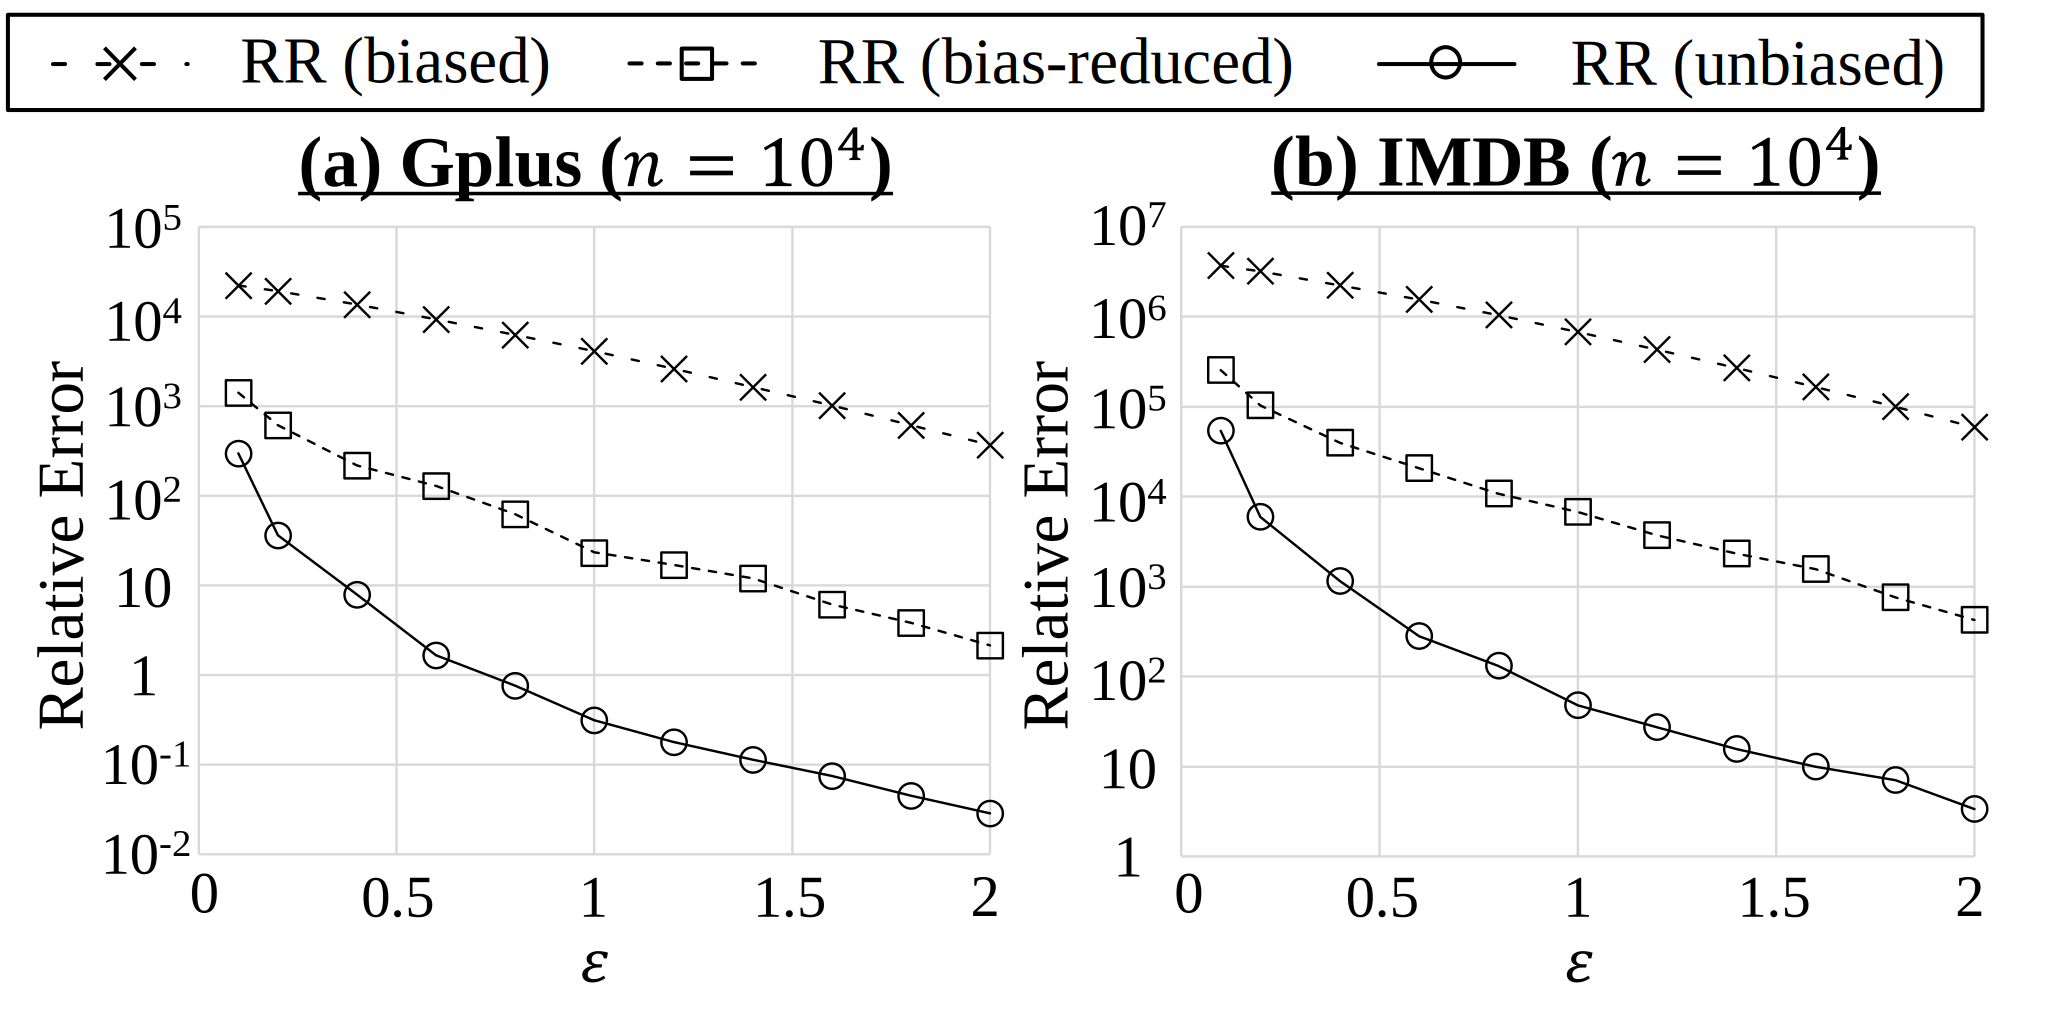
\includegraphics[width=0.99\linewidth]{fig/resB_one_round_small.pdf}
  
  \caption{Relative error of one-round algorithms for small datasets ($n=10000$).}
  \label{chap2-fig:resB_small}
\end{figure}

Figure~\ref{chap2-fig:resB_small} shows the results.
\textsf{RR (bias-reduced)} significantly outperforms \textsf{RR (biased)} and is significantly outperformed by \textsf{RR (unbiased)}.
We believe 
% that 
this is caused by the fact that \textsf{RR (bias-reduced)} introduces some approximation and does not calculate an unbiased estimate of $f_\triangle(G)$.

\smallskip
\noindent{\textbf{Large Datasets.}}~~Based on Figure~\ref{chap2-fig:resB_small}, we improve the time complexity of \textsf{RR (unbiased)} using the ARR and compare it with our two-rounds algorithms in large datasets.

Specifically, \textsf{RR (unbiased)} counts \textit{triangles}, \textit{$2$-edges} (three nodes with two edges), \textit{$1$-edges} (three nodes with one edge), and \textit{no-edges} (three nodes with no edges) in $G'$ obtained by Warner's RR.
Let $m_3, m_2, m_1, m_0 \in \nnints$ be the numbers of triangles, $2$-edges, $1$-edges, and no-edges, respectively, after applying Warner's RR.
\textsf{RR (unbiased)} calculates an unbiased estimate of $f_\triangle(G)$ from these four values.
Thus, we improve \textsf{RR (unbiased)} by using the ARR, which samples each edge with probability $p_2$ after Warner's RR, and then calculating unbiased estimates of $m_3$, $m_2$, $m_1$, and $m_0$.

Let $\hat{m}_3, \hat{m}_2, \hat{m}_1, \hat{m}_0 \in \reals$ be the unbiased estimates of $m_3$, $m_2$, $m_1$, and $m_0$, respectively. 
% after applying Warner's RR.
Let $m_3^*, m_2^*, m_1^*, m_0^* \in \nnints$ be the number of triangles, 2-edges, 1-edges, no-edges, respectively, after applying the ARR.
Since the ARR samples each edge with probability $p_2$, we obtain:
\begin{align*}
    m_3^* &= \textstyle{p_2^3 \hat{m}_3} \\
    m_2^* &= \textstyle{3p_2^2(1-p_2) \hat{m}_3 + p_2^2 \hat{m}_2} \\
    m_1^* &= \textstyle{3p_2(1-p_2)^2 \hat{m}_3 + 2p_2(1-p_2) \hat{m}_2 + p_2 \hat{m}_1.}
\end{align*}
By these equations,
% and $\hat{m}_3 + \hat{m}_2 + \hat{m}_1 + \hat{m}_0 = \frac{n(n-1)(n-2)}{6}$,
we obtain:
\begin{align}
    \hat{m}_3 &= \textstyle{\frac{m_3^*}{p_2^3}} \label{chap2-eq:hm_3} \\
    \hat{m}_2 &= \textstyle{\frac{m_2^*}{p_2^2} - 3(1-p_2)\hat{m}_3} \label{chap2-eq:hm_2} \\
    \hat{m}_1 &= \textstyle{\frac{m_1^*}{p_2} - 3(1-p_2)^2\hat{m}_3 - 2(1-p_2)\hat{m}_2} \label{chap2-eq:hm_1} \\
    \hat{m}_0 &= \textstyle{\frac{n(n-1)(n-2)}{6} - \hat{m}_3 - \hat{m}_2 - \hat{m}_1.} \label{chap2-eq:hm_0}
\end{align}
Therefore, after applying the ARR to the lower triangular part of $\bmA$, the server counts $m_3^*$, $m_2^*$, $m_1^*$, and $m_0^*$ in $G'$, and then calculates the unbiased estimates $\hat{m}_3$, $\hat{m}_2$, $\hat{m}_1$, and $\hat{m}_0$ by (\ref{chap2-eq:hm_3}), (\ref{chap2-eq:hm_2}), (\ref{chap2-eq:hm_1}), and (\ref{chap2-eq:hm_0}), respectively.
Finally, the server estimates $f_\triangle(G)$ from $\hat{m}_3$, $\hat{m}_2$, $\hat{m}_1$, and $\hat{m}_0$ in the same way as \textsf{RR (unbiased)}.
We denote this algorithm by \textsf{ARR (unbiased)}.
The time complexity of \textsf{ARR (unbiased)} is $O(\mu^3 n^3)$, where $\mu$ is the ARR parameter.

We compared \textsf{ARR (unbiased)} with our three algorithms with double clipping using \GPlus{} ($n=107614$) and \IMDB{} ($n=896308$).
For the sampling probability $p_2$, we set $p_2 = 10^{-3}$ or $10^{-6}$.
We averaged the relative error over $10$ runs.

\begin{figure}[t]
  \centering
  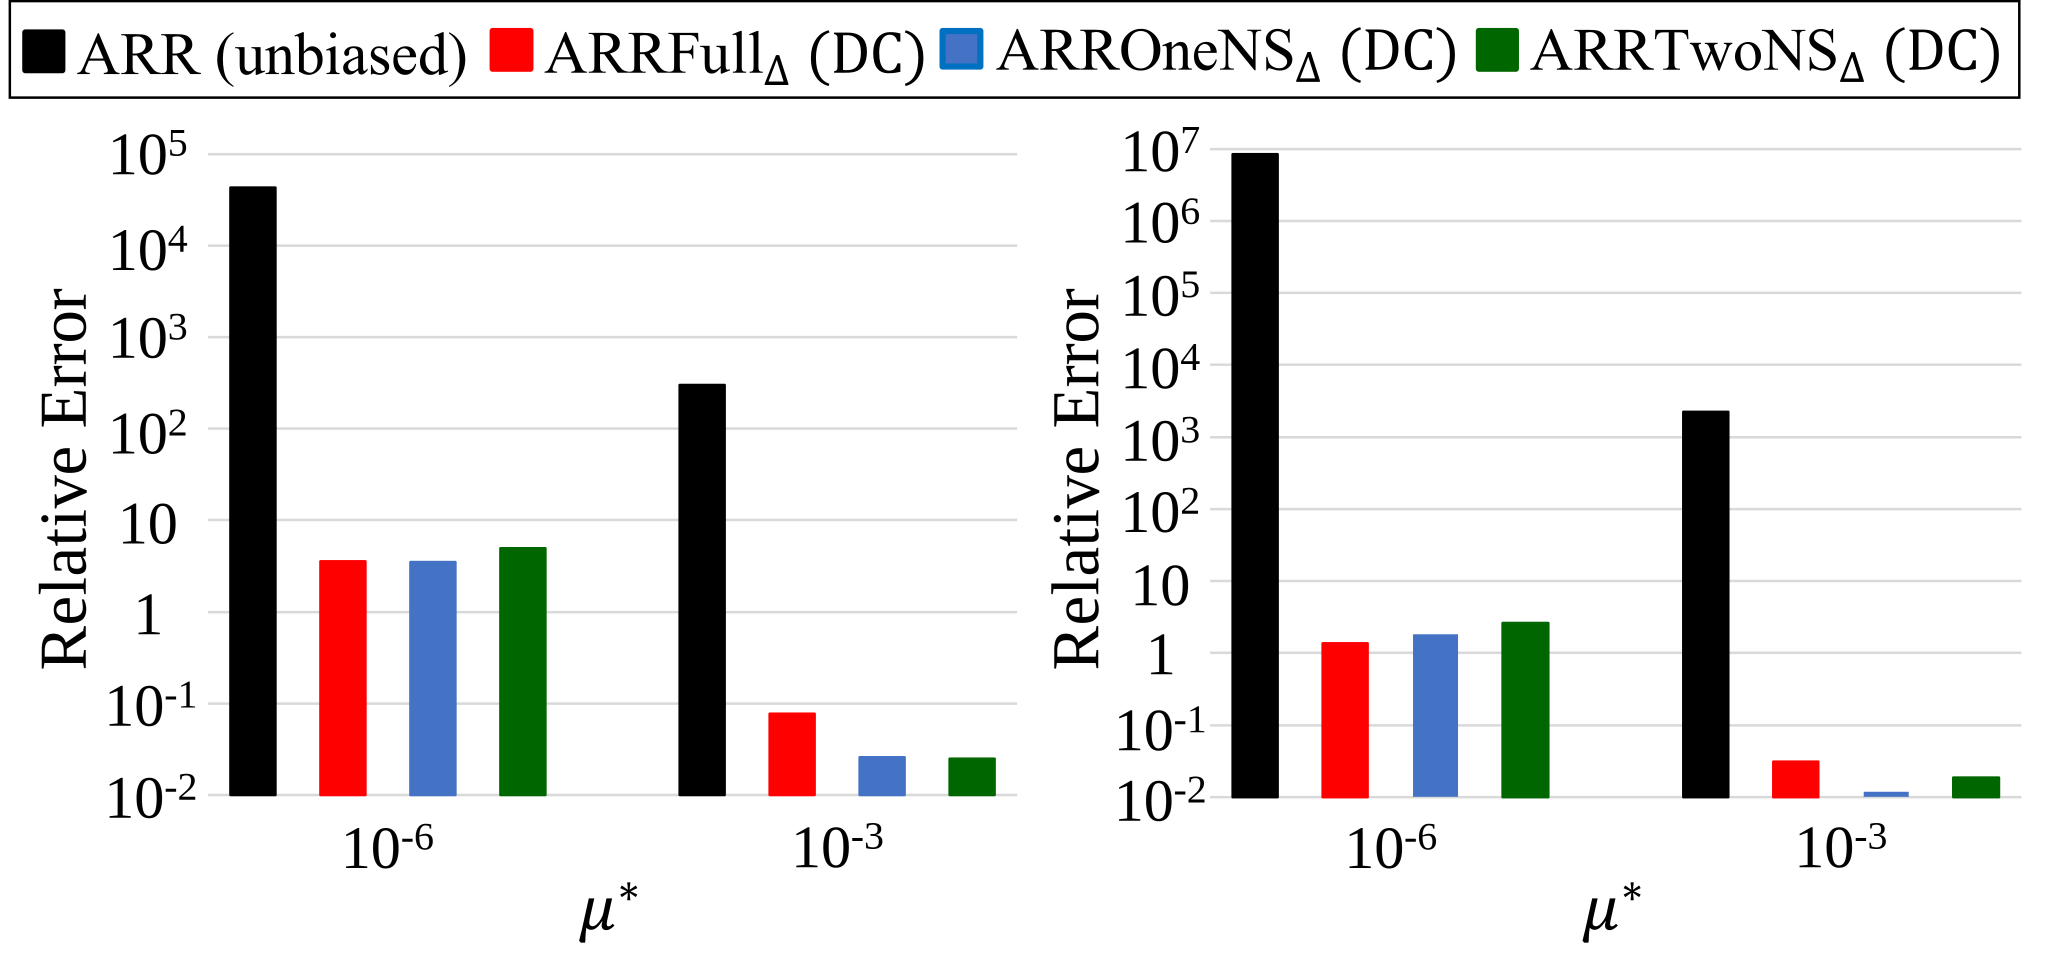
\includegraphics[width=0.99\linewidth]{fig/resB_one_round_large.pdf}
  
  \caption{Relative error of the one-round algorithm \textsf{ARR (unbiased)} and our three two-rounds algorithms with double clipping for large datasets ($n=107614$ in \GPlus{}, $n=896308$ in \IMDB{}).}
  \label{chap2-fig:resB_large}
\end{figure}

Figure~\ref{chap2-fig:resB_large} shows the results, where we set
% $\mu_F$ ($=\mu_o^2=\mu_T^3$)
$\mu^* = 10^{-6}$ or $10^{-3}$.
In \textsf{ARR (unbiased)}, we used $\mu^*$ as 
% a parameter $\mu$ of the ARR.
the ARR parameter $\mu$. 
Thus, we can see \textit{how much the relative error is reduced by introducing an additional round with \AlgOne{}}.
Figure~\ref{chap2-fig:resB_large} shows that the relative error of \textsf{ARR (unbiased)} is prohibitively large; i.e., relative error $\gg 1$.
% even when $\mu_F = 10^{-3}$.
This is because three edges are noisy in any noisy triangle. 
% and edge sampling is introduced to reduce the time complexity. 
% (recall that the one-round algorithms without sampling would require about $35$ years when $n=10^6$ \cite{Imola_USENIX21}).
% The relative error is extremely large when $\mu_F = 10^{-6}$ due to a very small sampling probability.
The relative error is significantly reduced by  introducing an additional round
% and counting noisy triangles in which only one edge is noisy.
% In contrast, our algorithms achieve much smaller estimation error
because only one edge is noisy in each noisy triangle at the second round.

In summary, one-round algorithms are far from acceptable in terms of the estimation error for large graphs, and two-round algorithms such as ours are necessary.

\section{Clustering Coefficient}
\label{chap2-sec:cluster}
% \smallskip
% \noindent{\textbf{Clustering Coefficient.}}~~We
Here we
% We have so far evaluated the estimation error of the triangle count.
% finally
% show that our algorithms are very useful for estimating the clustering coefficient.
evaluate the estimation error of the clustering coefficient using our algorithms.

% evaluated the estimation error of the clustering coefficient as follows.
We first estimated a triangle count by using our \AlgTwo{} with double clipping
($\epsilon_0 = \frac{\epsilon}{10}$ and
$\epsilon_1 = \epsilon_2 = \frac{9\epsilon}{20}$)
because it provides the best performance in Figures~\ref{chap2-fig:res2_w_Lap_abst}, \ref{chap2-fig:res2_w_Lap}, and \ref{chap2-fig:res3_n}.
Then we estimated a $2$-star count by
% a modified version of the algorithm in~\cite{Imola_USENIX21} using the adaptive edge clipping in Section~\ref{chap2-sec:double_clip}.
using the one-round $2$-star algorithm in~\cite{Imola_USENIX21} with the
% adaptive
edge clipping in Section~\ref{chap2-sec:double_clip}.

Specifically, we calculated a noisy degree $\td_i$ of each user $v_i$ 
% (possibly with edge clipping) 
by using the edge clipping with the privacy budget $\epsilon_0$.
Then we calculated the number $r_i \in \nnints$ of $2$-stars of which user $v_i$ is a center, and added $\Lap(\frac{\Delta}{\epsilon_1})$ to $r_i$, where $\Delta = \binom{\td_i}{2}$.
Let $\hr_i = r_i + \Lap(\frac{\Delta}{\epsilon_1})$ be the noisy $2$-star of $v_i$.
Finally, we calculated
% the sum of the noisy $2$-stars
the sum $\sum_{i=1}^n \hr_i$ as an estimate of the $2$-star count.
This $2$-star algorithm provides ($\epsilon_0 + \epsilon_1$)-edge privacy (see~\cite{Imola_USENIX21} for details).
For the privacy budgets $\epsilon_0$ and $\epsilon_1$, we set $\epsilon_0 = \frac{\epsilon}{10}$ and $\epsilon_1 = \frac{9\epsilon}{10}$.

Based on the triangle and $2$-star counts, we estimated the clustering coefficient as
$\frac{3 \times \hf_\triangle(G)}{\hf_{2\star}(G)}$,
% $3 \times \hf_\triangle(G) / \hf_{2\star}(G)$,
where $\hf_\triangle(G)$ (resp.~$\hf_{2\star}(G)$) is the estimate of the triangle (resp.~$2$-star) count.

\begin{figure}[t]
  \centering
  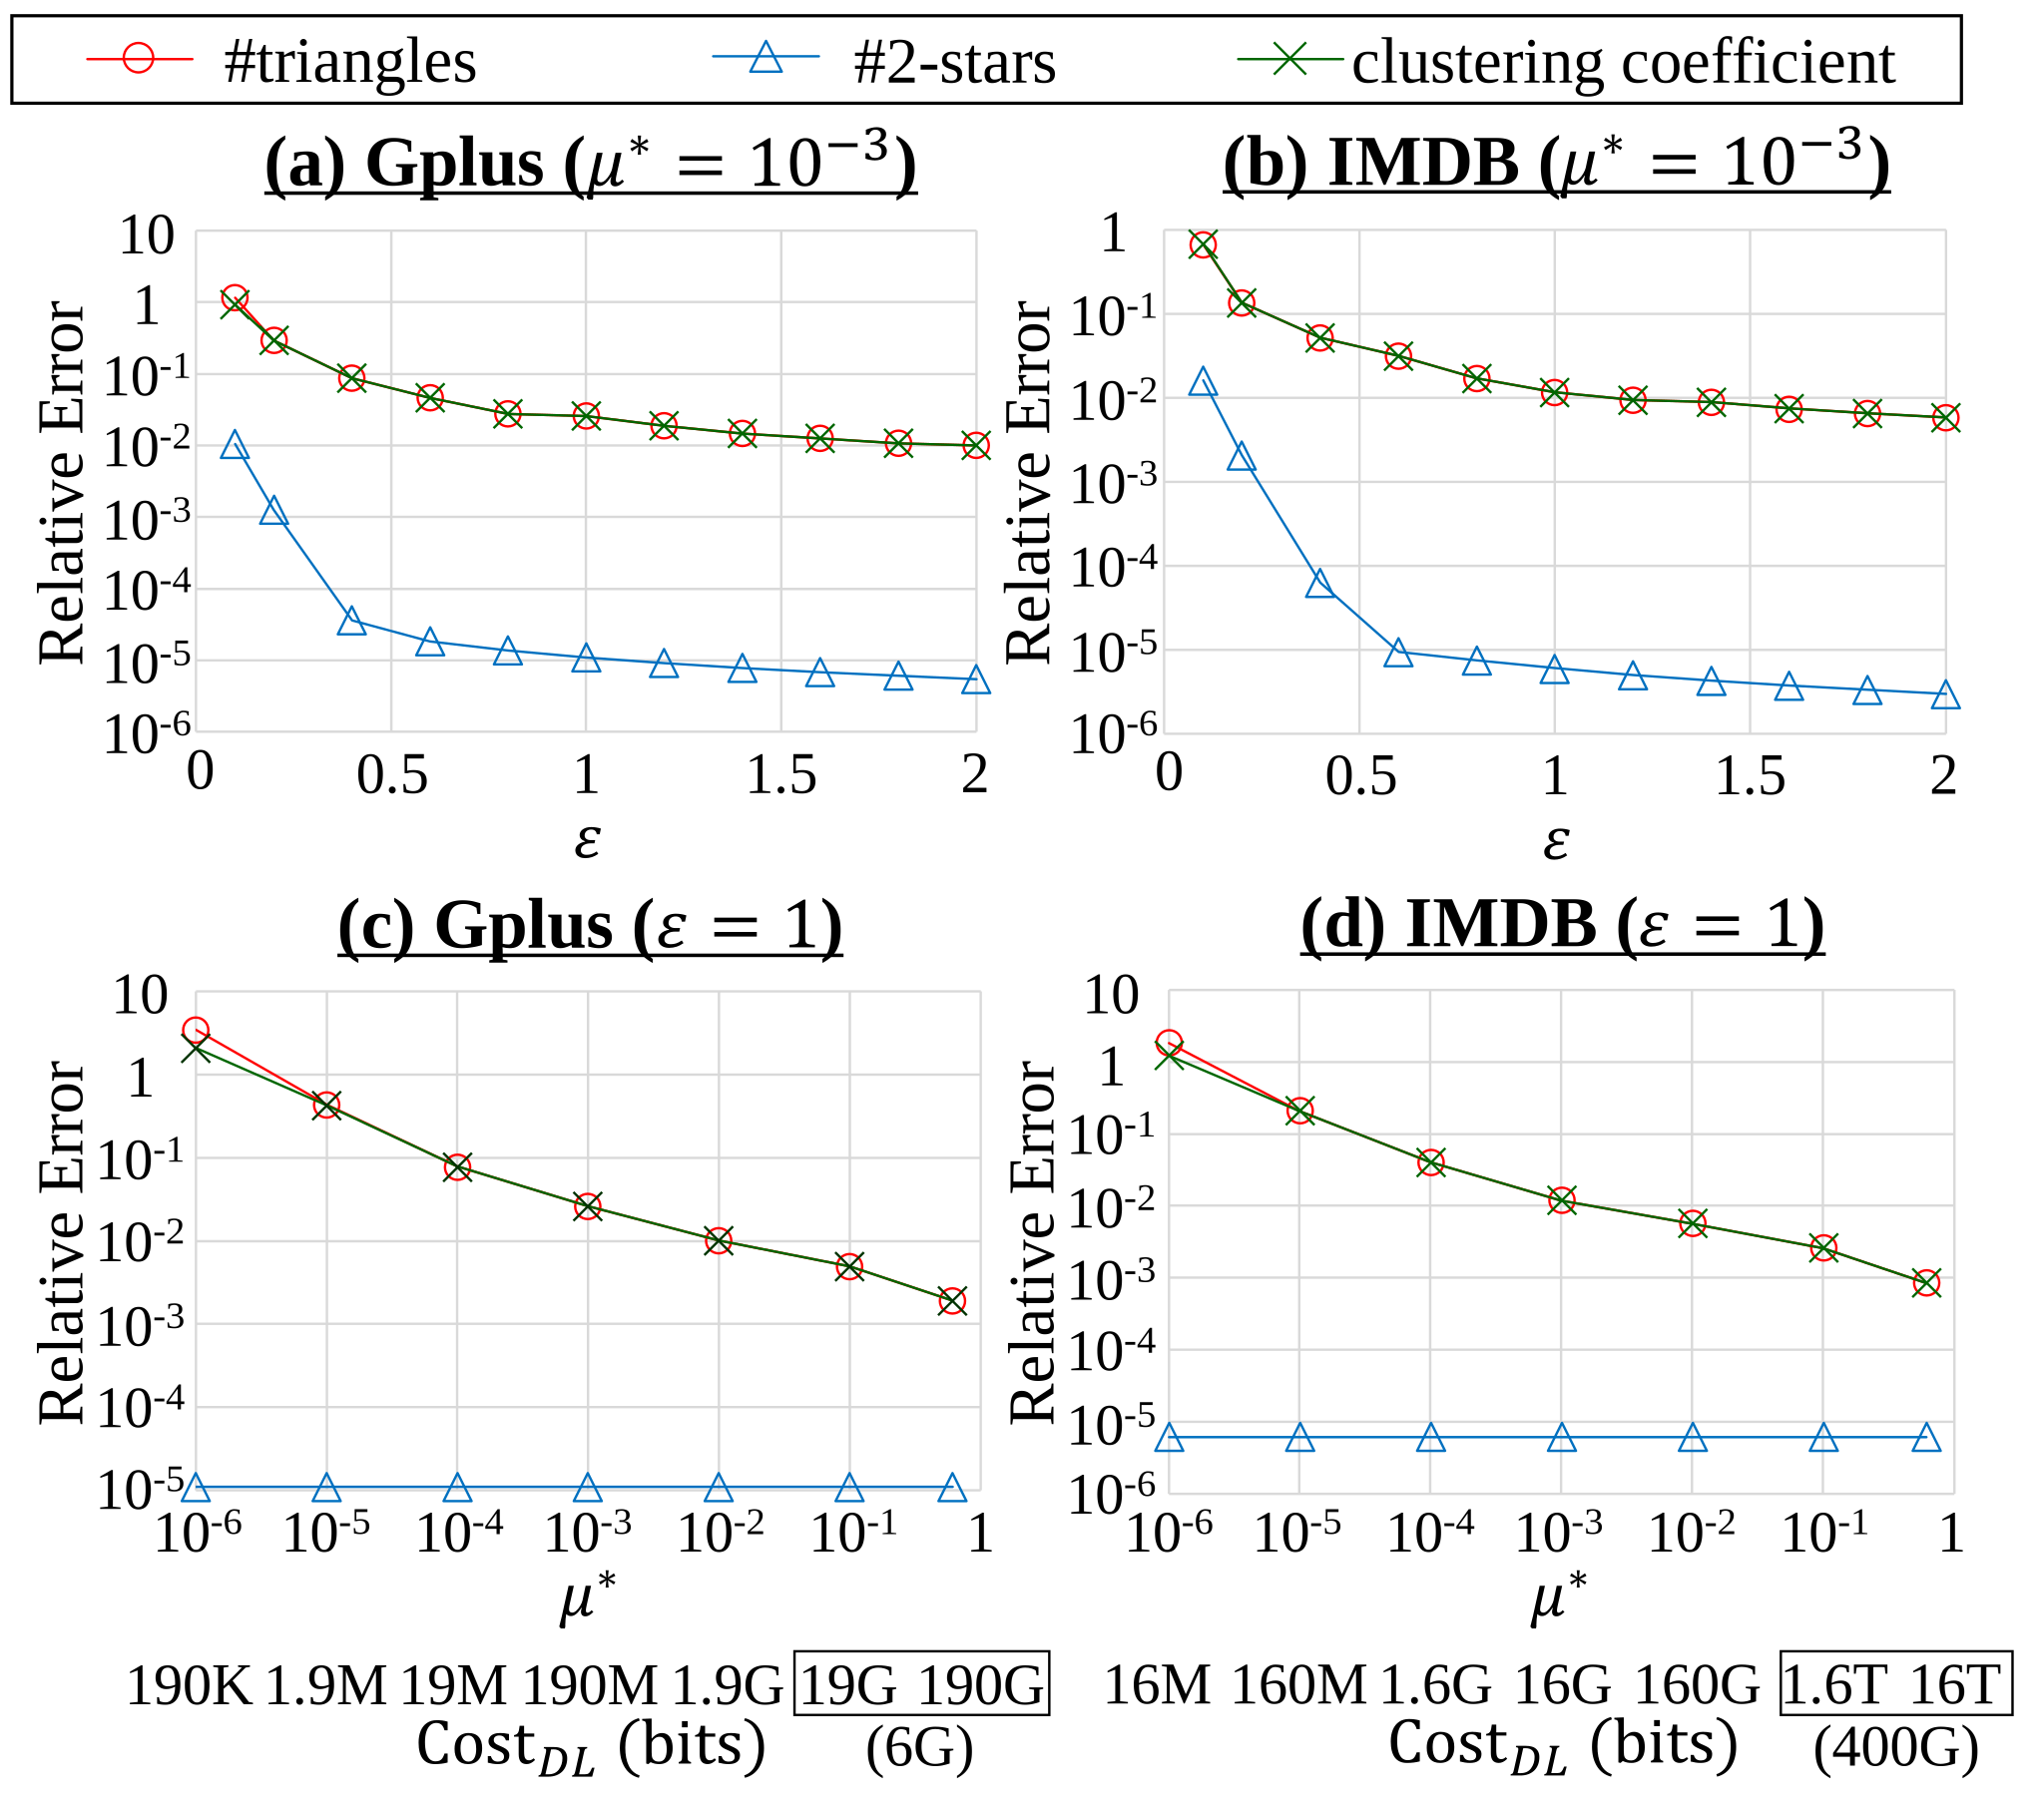
\includegraphics[width=0.99\linewidth]{fig/res5_cluster.pdf}
  
  \caption{Relative errors of \#triangles, \#$2$-stars, and the clustering coefficient in \AlgTwo{} with double clipping.
  $\CostDL$ is calculated by (\ref{chap2-eq:CostDL_F})
  (when $\mu^* \geq 0.1$,
  $\CostDL$ can be $6$ Gbits and $400$ Gbits in \GPlus{} and \IMDB{}, respectively).
  }
  \label{chap2-fig:res5_cluster}
\end{figure}

Figure~\ref{chap2-fig:res5_cluster} shows the relative errors of the triangle count, $2$-star count, and clustering coefficient.
Note that the relative error of the 2-star count is not changed by changing
% $\mu_F$ ($=\mu_O^2=\mu_T^3$)
$\mu^*$
because the 2-star algorithm does not use the ARR.
Figure~\ref{chap2-fig:res5_cluster} shows that the relative error of the $2$-star count is much smaller than that of the triangle count.
This is because each user can count her 2-stars locally (whereas she cannot count her triangles), as described in Section~\ref{chap2-sec:intro}.
Consequently, the relative error of the clustering coefficient is almost the same as that of the triangle count, as the denominator $\hf_{2\star}(G)$ in the clustering coefficient is very accurate.

Note that the clustering coefficient requires the privacy budgets for
calculating both $\hf_\triangle(G)$ and $\hf_{2\star}(G)$
% both the triangle count and $2$-star count
(in Figure~\ref{chap2-fig:res5_cluster}, $2\epsilon$ in total).
% $2\epsilon$ because it needs both the triangle count and $2$-star count.
However, we can accurately
% estimate the $2$-star count
calculate $\hf_{2\star}(G)$
with a very small privacy budget, as shown in Figure~\ref{chap2-fig:res5_cluster}.
Thus, we can accurately estimate the clustering coefficient with almost the same privacy budget as
the triangle count
% $\hf_\triangle(G)$
% by making the privacy budget for the $2$-star count small (e.g., $\epsilon=0.1$ or $0.2$).
by assigning a very small privacy budget (e.g., $\epsilon=0.1$ or $0.2$) for
% the $2$-star count.
$\hf_{2\star}(G)$.

In summary, we can accurately estimate the clustering coefficient as well as the triangle count under edge LDP by using our \AlgTwo{} with double clipping.

\arxiv{
\section{Experiments Using the Barab\'{a}si-Albert Graph Datasets}
\label{chap2-sec:BAmodel}
In Section~\ref{chap2-sec:experiments}, we evaluated our algorithms using two real datasets.
Below we also evaluate our algorithms using a synthetic graph based on the BA (Barab\'{a}si-Albert) graph model~\cite{NetworkScience}, which has a power-law degree distribution.

In the BA graph model, a graph of $n$ nodes is generated by attaching new nodes one by one.
% Each node has $m \in \nnints$ edges, 
Each new node is connected to $m \in \nnints$ existing nodes, 
and each edge is connected to an existing node with probability proportional to its degree.
We used NetworkX \cite{Hagberg_SciPy08}, a Python package for complex networks, to generate synthetic graphs based on the BA graph model.

We generated a graph $G=(V,E)$ with the same number of nodes as
% the Google+ dataset~\cite{McAuley_NIPS12} (\GPlus{});
\GPlus{}; i.e., $n=107614$ nodes.
% and $m=$
For the number $m$ of edges per node, we set $m=50$, $114$, or $500$.
% Note that the BA graph with $m=114$ has almost the average degree as \GPlus{}.
% When $m=114$, most nodes have the degree of $114$, which is the average degree in \GPlus{}. 
% Thus, we can see the difference between them.
Using these graphs, we evaluated our three algorithms with double clipping.
We set parameters in the same as Section~\ref{chap2-sec:experiments}; i.e.,
$\alpha = 150$, $\beta = 10^{-6}$, $\epsilon_0 = \frac{\epsilon}{10}$, and $\epsilon_1 = \epsilon_2 = \frac{9\epsilon}{20}$.
% We ran each algorithm $10$ times, and averaged the relative error over the $10$ cases.
For each algorithm, we averaged the relative error over $10$ runs.

% \begin{figure}[t]
%   \centering
%   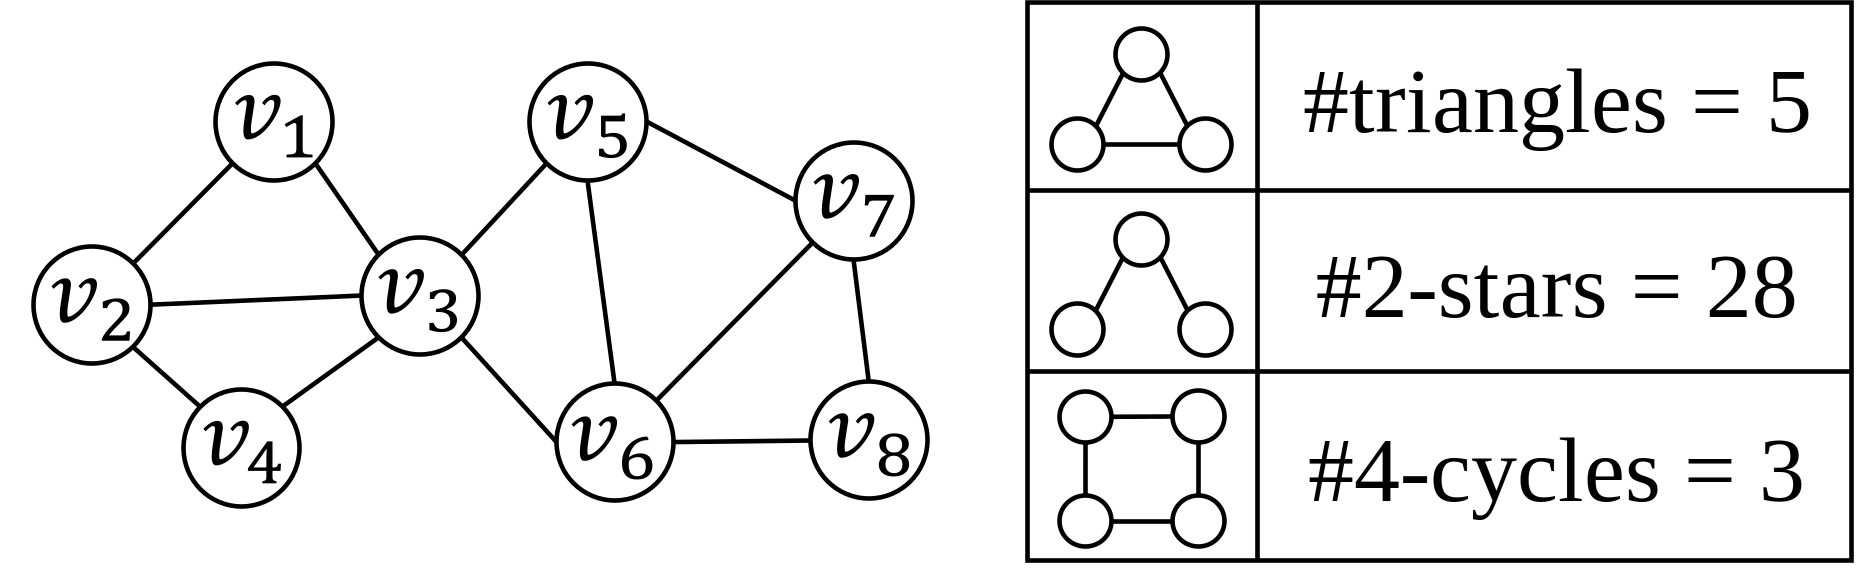
\includegraphics[width=0.95\linewidth]{fig/subgraphs.pdf}
%   
%   \caption{Subgraphs used in our theoretical analysis.}
%   \label{chap2-fig:subgraphs}
% \end{figure}

Figure~\ref{chap2-fig:resA_BAGraph} shows the results, where $\epsilon=1$ and
% $\mu_F$ ($= \mu_O^2 = \mu_T^3$)
$\mu^* = 10^{-3}$.
We observe that \AlgTwo{} significantly outperforms \AlgOne{} and \AlgThree{} when $m=500$, and that \AlgTwo{} performs almost the same as \AlgOne{} when $m=50$ or $114$.

To examine the reason for this, we also decomposed the estimation error into two components (the first error by empirical estimation and the second error by the Laplacian noise) in the same way as Figure~\ref{chap2-fig:res3_emp_Lap}.
Figure~\ref{chap2-fig:resA_BAGraph_emp_Lap} shows the results.
% In addition, we calculated the number $C_4$ of $4$-cycles in the BA graph.
We also show in Table~\ref{chap2-tab:resA_4cycles} the number $C_4$ of $4$-cycles in each BA graph ($m=50$, $114$, or $500$) and \GPlus{}.

From Figure~\ref{chap2-fig:resA_BAGraph_emp_Lap} and Table~\ref{chap2-tab:resA_4cycles}, we can explain Figure~\ref{chap2-fig:resA_BAGraph} as follows.
The BA graphs with $m=50$ and $114$ have a much smaller number $C_4$ of $4$-cycles than \GPlus{}, as shown in Table~\ref{chap2-tab:resA_4cycles}.
Consequently,
% the error caused by
the Laplacian noise is relatively large and dominant for these two graphs, as shown in Figure~\ref{chap2-fig:resA_BAGraph_emp_Lap}.
In particular,
% the relative error of
the Laplacian noise is the largest in \AlgThree{} because it cannot effectively reduce the global sensitivity by double clipping, as explained in Section~\ref{chap2-sec:double_clip}.
In contrast, the BA graph with $m=500$ has a larger number $C_4$ of $4$-cycles than \GPlus{}, and therefore the Laplacian noise is not dominant (except for \AlgThree{}).
This explains the results in Figure~\ref{chap2-fig:resA_BAGraph}.

These results
% , along with Section~\ref{chap2-sec:experiments},
% Our experimental results in Appendix~\ref{chap2-sec:BAmodel} and Section~\ref{chap2-sec:experiments},
show that \AlgTwo{} outperforms \AlgOne{} especially when the number $C_4$ of $4$-cycles is large.
As we have shown in Section~\ref{chap2-sec:experiments} and Appendix~\ref{chap2-sec:BAmodel}, $C_4$ is large in a large graph (e.g., $n \approx 10^6$) or dense graph (e.g., \GPlus{}, BA graph with $m=500$).

\begin{figure}[t]
  \centering
  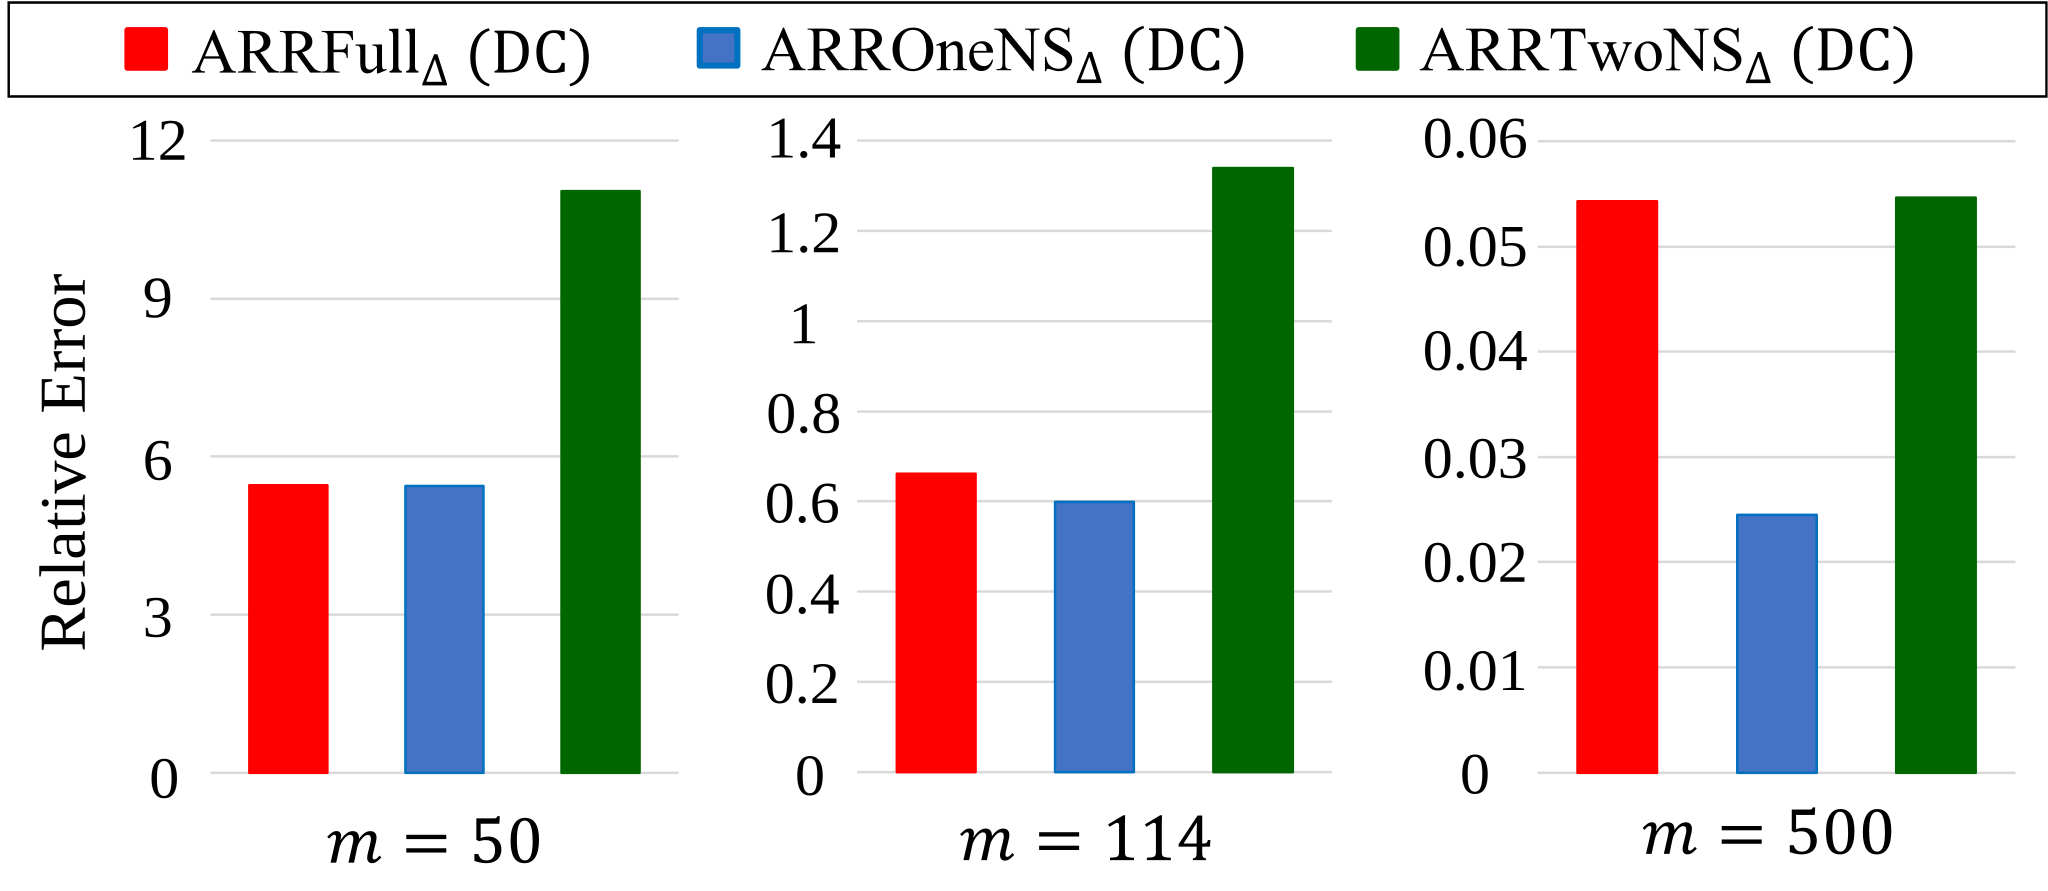
\includegraphics[width=0.99\linewidth]{fig/resA_BAGraph.pdf}
  
  \caption{Relative error of our three algorithms with double clipping in the BA graphs ($n=107614$, $\epsilon=1$, $\mu^* = 10^{-3}$).}
  \label{chap2-fig:resA_BAGraph}
% \end{figure}
\vspace{5mm}
% \begin{figure}[t]
  \centering
  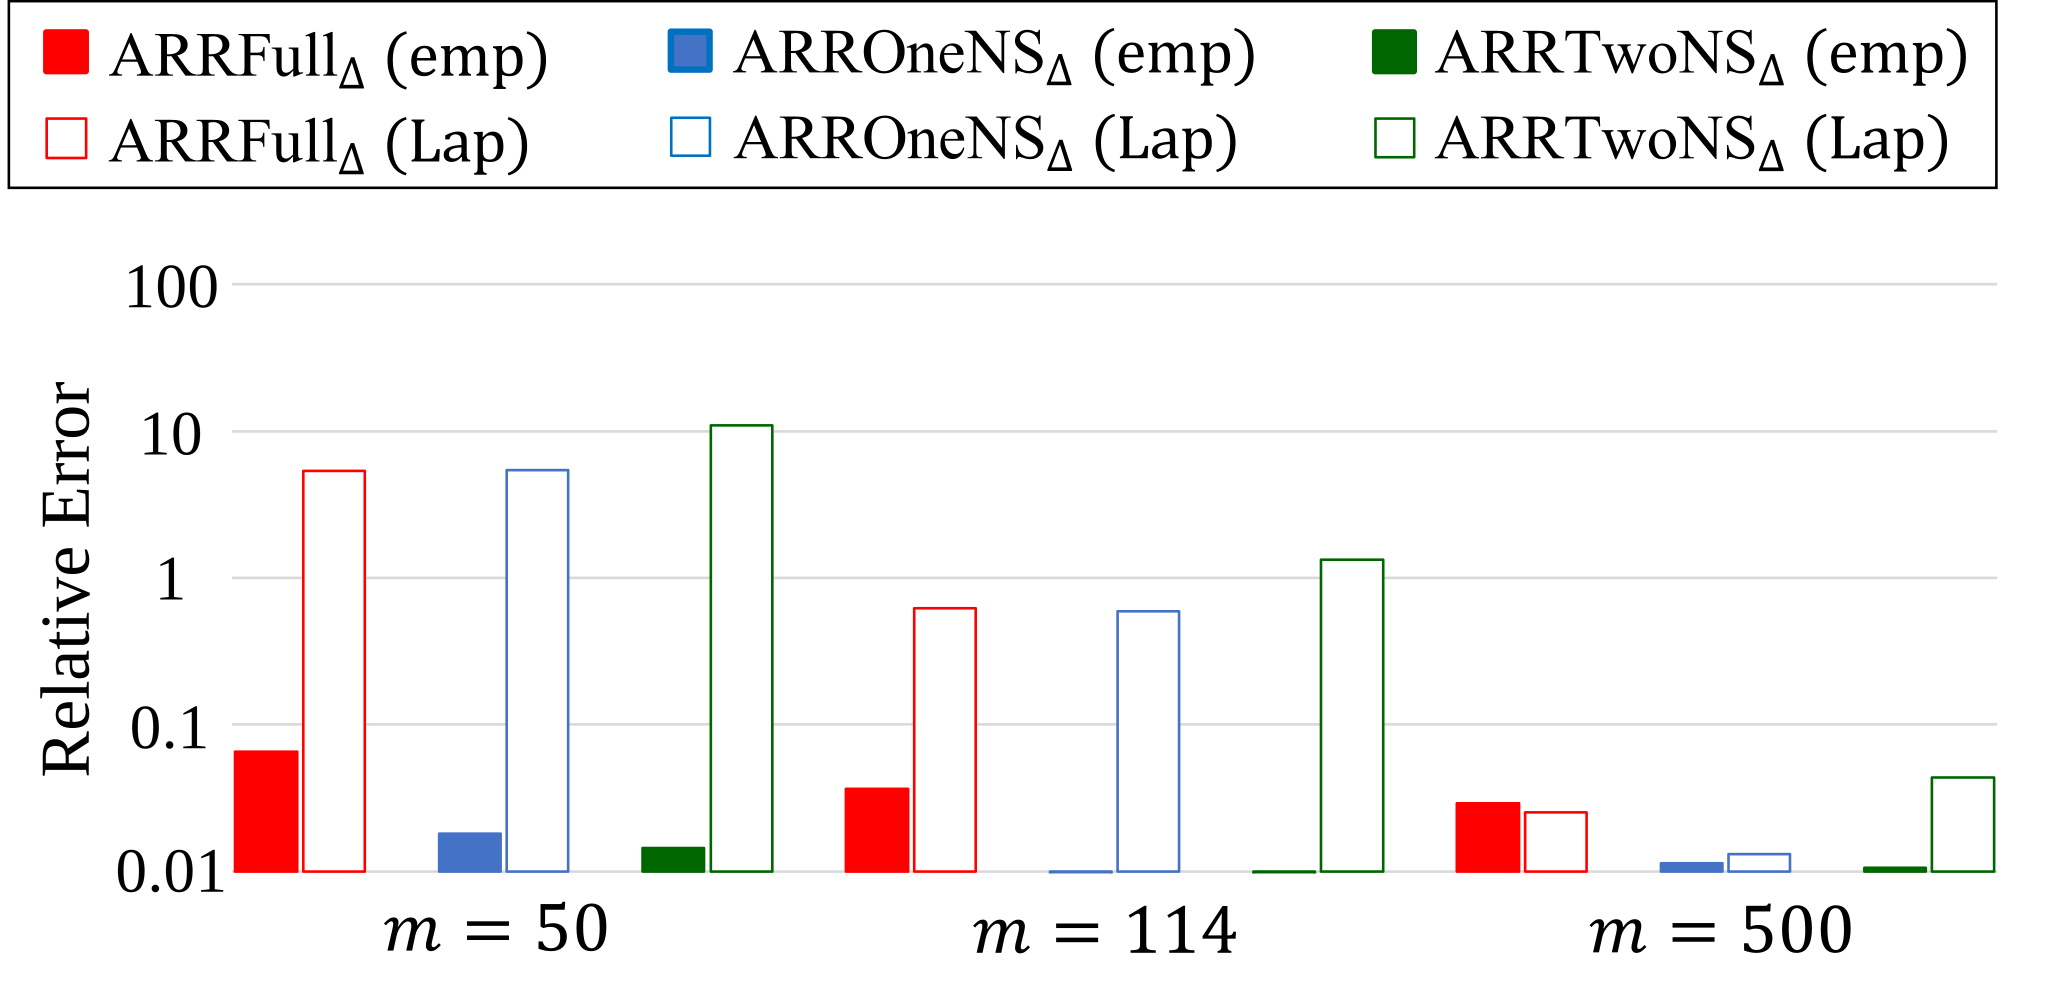
\includegraphics[width=0.95\linewidth]{fig/resA_BAGraph_emp_Lap.pdf}
  
  \caption{Relative error of empirical estimation and the Laplacian noise in our three algorithms with double clipping in the BA graphs ($n=107614$, $\epsilon=1$, $\mu^* = 10^{-3}$).}
  \label{chap2-fig:resA_BAGraph_emp_Lap}
\end{figure}

\section{Edge Clipping and Noisy Triangle Clipping}
\label{chap2-sec:EC_DC}
% \smallskip
% \noindent{\textbf{Edge Clipping and Noisy Triangle Clipping.}}~~
In Section~\ref{chap2-sec:experiments}, we showed that our double clipping significantly reduces the estimation error.
To investigate the effect of
% adaptive
edge clipping and noisy triangle clipping independently, we also performed the following ablation study.

We evaluated our three algorithms with only
% adaptive
edge clipping; i.e., each user calculates a noisy degree $\td_i$ (possibly with edge clipping) and then adds $\Lap(\frac{\td_i}{\epsilon_2}$) to her noisy triangle count.
Then we compared them with our algorithms with double clipping and without clipping.

\begin{table}[t]
\caption{\#$4$-cycles $C_4$ in each graph dataset.}
\centering
\hbox to\hsize{\hfil
\begin{tabular}{l|l|l|l|l}
\hline
		&	$m=50$   &  $m=114$   &  $m=500$   &  \GPlus{}\\
\hline
$C_4$   &   $8.8 \times 10^8$ &  $1.7 \times 10^{10}$ &   $3.1 \times 10^{12}$ &   $2.8 \times 10^{12}$\\
\hline
\end{tabular}
\hfil}
\label{chap2-tab:resA_4cycles}
\end{table}

\begin{figure}[t]
  \centering
  \includegraphics[width=0.99\linewidth]{fig/res2_w_Lap_EC.pdf}
  
  \caption{Relative error of our three algorithms without clipping (``$d_{max}$''), with only edge clipping (``EC''), and double clipping (``DC'') when $\epsilon=1$ and $\mu^* = 10^{-6}$ or $10^{-3}$ ($n=107614$ in \GPlus{}, $n=896308$ in \IMDB{}).}
  \label{chap2-fig:res2_w_Lap_EC}
\end{figure}

Figure~\ref{chap2-fig:res2_w_Lap_EC} shows the results, where $\epsilon=1$, $\mu^* = 10^{-6}$ or $10^{-3}$, and ``EC'' represents our algorithms with only
% adaptive
edge clipping.
We observe that ``EC''
% (only edge clipping)
outperforms ``$d_{max}$'' (w/o clipping) and is outperformed by ``DC'' (double clipping).
The difference between ``EC'' and ``DC'' is significant especially when $\mu^* = 10^{-6}$ (``DC'' is smaller than $\frac{1}{100}$ of ``EC'').
This is because our noisy triangle clipping reduces the global sensitivity by using a small value of
$\mu^*$. 
% $\mu_F$ ($=\mu_O^2 = \mu_T^3$).
From Figure~\ref{chap2-fig:res2_w_Lap_EC}, we conclude that each component (i.e.,
% adaptive
edge clipping, noisy triangle clipping) is essential in our double clipping.

\section{Proof of Proposition~\ref{chap2-prop:seq_comp_edge_LDP}}
\label{chap2-sec:proof_seq_comp_edge_LDP}
Let $\calR_i(\bma_i) = (\calR_i^1(\bma_i), \calR_i^2(M_i)(\bma_i))$ be the
randomizer used by user $v_i$ in the composition. To establish that
$\calR_i(\bma_i)$ satisfies $\epsilon$-edge LDP for every $v_i \in V$, we will
prove that~\eqref{chap2-eq:edge_LDP} holds for $\calR_i(\bma_i)$. To do this, first write
\begin{align*}
  &\;\Pr[(\calR_i^1(\bma_i), \calR_i^2(M_i)(\bma_i)) = (r_i^1, r_i^2)] = \\
  &\qquad\Pr[\calR_i^1(\bma_i) = r_i^1]\Pr[\calR_i^2(M_i)(\bma_i) = r_i^2 | \calR_i^1(\bma_i) = r_i^1] \\
  &\qquad\Pr[\calR_i^1(\bma_i) = r_i^1]\Pr[\calR_i^2(M_i)(\bma_i) = r_i^2 | M_i = \lambda_i(r_i^1)],
\end{align*}
where the last equality follows because $M_i = \lambda_i(\calR_i^1(\bma_i))$ for a post-processing algorithm $\lambda_i$.
Notice that the same equalities are true when we replace $\bma_i$ with $\bma_i'$.
Because $\calR_i^1$ and $\calR_i^2(M_i)$ (for any $M_i$) satisfy $\epsilon_1, \epsilon_2$-edge LDP, respectively,
we have
\begin{align*}
  &\;\Pr[\calR_i^1(\bma_i) = r_i^1]\Pr[\calR_i^2(M_i)(\bma_i) = r_i^2 | M_i = \lambda_i(r_i^1)] \\
  &\qquad\leq e^{\epsilon_1}\Pr[\calR_i^1(\bma_i') = r_i^1]e^{\epsilon_2}\Pr[\calR_i^2(\bma_i') = r_i^2 | M_i = \lambda_i(r_i^1)] \\
  &\qquad= e^{\epsilon_1 + \epsilon_2} \Pr[(\calR_i^1(\bma_i'), \calR_i^2(M_i)(\bma_i')) = (r_i^1, r_i^2)].
\end{align*}
This establishes the result. \qed

\section{Proof of Statements in Section~\ref{chap2-sec:algorithms}}
\label{chap2-sec:proof_algorithms}
\subsection{Proof of Theorem~\ref{chap2-thm:privacy_algorithms}}
Let $\bma_i, \bma'_i \in \{0,1\}^n$ be two neighbor lists that differ in one bit.
Let $t'_i$, $s'_i$, and $w'_i$ be respectively the values of $t_i$ (line 11 of Algorithm~\ref{chap2-alg:unify}), $s_i$ (line 12), and $w_i$ (line 13) when the neighbor list of user $v_i$ is $\bma'_i$.
Let $\Delta w_i = |w'_i - w_i|$.
Then we have $t'_i - t_i \in [0,d_{max}]$ and $s'_i - s_i \in [0,d_{max}]$, and therefore $\Delta w_i = |(t'_i - t_i) - \mu^* \rho(s'_i - s_i)| \leq d_{max}$.

Since we add
$\Lap\left(\frac{d_{max}}{\epsilon_2}\right)$
to $w_i$, the second round provides $\epsilon_2$-edge LDP.
The first round uses $ARR_{\epsilon_1,\mu}$ and provides $\epsilon_1$-edge LDP.
Thus, by sequential composition (Proposition~\ref{chap2-prop:seq_comp_edge_LDP}),
Algorithm~\ref{chap2-alg:unify} provides ($\epsilon_1+\epsilon_2$)-edge LDP in total.
It also provides ($\epsilon_1+\epsilon_2$)-relationship DP because it uses only the lower-triangular part of $\bmA$ (Proposition~\ref{chap2-prop:edge_LDP_entire_edge_LDP}).
% \ji{We should formally state the lower-triangular relationship DP result somewhere, I think maybe add it to proposition 1.}
\qed

\subsection{Proof of Theorem~\ref{chap2-thm:l2loss_algorithms}}
\label{chap2-sub:prrof_l2loss_algorithms}
% \paragraph{Unbiased Estimators}
% \smallskip
\noindent{\textbf{Unbiased Estimators.}}~~First, we will show that $\hf_\triangle(G)$ satisfies
$\E[\hf_\triangle(G)] = f_\triangle(G)$ for all $G \in \calG$, in \AlgOne{}, \AlgTwo{}, \AlgThree{}.
Regardless of algorithm, we have
\begin{align}
  &\;\E[\hf_\triangle(G)] \nonumber \\
  &= \frac{1}{\mu^*(1-\rho)}\sum_{i=1}^n \E[w_i] \nonumber \\
  &= \frac{1}{\mu^*(1-\rho)}\sum_{i=1}^n \E[t_i - \mu^* \rho s_i] \nonumber \\
  &= \frac{1}{\mu^*(1-\rho)}\sum_{i=1}^n \sum_{\substack{1 \leq j < k < i \leq n \\ a_{i,j} = a_{i,k} = 1}} \E[\textbf{1}_{(v_j, v_k) \in M_i} - \mu^* \rho],
  \label{chap2-eq:unbias_1}
\end{align}
where $\rho = e^{-\epsilon_1}$, and the quantites $\mu^*, t_i, s_i$ are defined in
Algorithm~\ref{chap2-alg:unify}. Given that $a_{i,j} = a_{i,k} = 1$, we have that
$\Pr[(v_i, v_j) \in E'] = \Pr[(v_i, v_k) \in E'] = \mu$ by definition of ARR.
Furthermore,
% $\Pr[(v_i, v_k) \in E'] = \mu$ if $a_{i,k} = 1$, and $\Pr[(v_i, v_k) \in E'] = \mu\rho$ otherwise.
$\Pr[(v_j, v_k) \in E'] = \mu$ if $a_{j,k} = 1$, and $\Pr[(v_j, v_k) \in E'] = \mu\rho$ otherwise.
Examining~\eqref{chap2-eq:M_i_I},~\eqref{chap2-eq:M_i_II}, and~\eqref{chap2-eq:M_i_III}, we have
\[
  \Pr[(v_j, v_k) \in M_i] =
  \begin{cases}
    \mu^* & a_{j,k} = 1 \\
    \mu^*\rho & a_{j,k} = 0
  \end{cases}
\]
for all the three algorithms (note that $\mu^* = \mu$, $\mu^2$, and $\mu^3$ in \AlgOne{}, \AlgTwo{}, \AlgThree{}, respectively).
Thus, $\E[\textbf{1}_{(v_j, v_k) \in M_i}] = \mu^* (\rho + (1-\rho) a_{j,k})$
($= \mu^*$ if $a_{i,j}=1$ and $\mu^* \rho$ if $a_{i,j}=0$).
Plugging into~\eqref{chap2-eq:unbias_1}, we have
\begin{align*}
  &\;\E[\hf_\triangle(G)] \\
  &=
  \frac{1}{\mu^*(1-\rho)}\sum_{i=1}^n \sum_{\substack{1 \leq j < k < i \leq n \\ a_{i,j} = a_{i,k} =
  1}} \mu^*(\rho + (1-\rho)a_{j,k}) - \mu^* \rho \\
  &= \frac{1}{\mu^*(1-\rho)}\sum_{i=1}^n \sum_{\substack{1 \leq j < k < i \leq n \\ a_{i,j} = a_{i,k} =
  1}} \mu^*(1-\rho)a_{j,k} \\
  &= \sum_{i=1}^n \sum_{\substack{1 \leq j < k < i \leq n \\ a_{i,j} = a_{i,k} =
  1}} a_{j,k} \\
  &= f_\triangle(G).
\end{align*} 
Thus, $\hf_\triangle(G)$ is unbiased. \qed

% \paragraph{$l_2^2$-Loss of Estimators}
\smallskip
\noindent{\textbf{$l_2$ Loss of Estimators.}}~~Using bias-variance decomposition, we have
for any graph $G$,
\begin{align*}
  l_2^2(f_\triangle(G), \hf_\triangle(G)) &= \E[(\hf_\triangle(G) - f_\triangle(G))^2] \\
  &= \E[(f_\triangle(G) - \E[\hf_\triangle(G)])^2] + \V[\hf_\triangle(G)] \\
  &= \V[\hf_\triangle(G)],
\end{align*}
where the last step follows because $\hf$ is unbiased.
Since $\hf_\triangle(G) = \frac{1}{\mu^*(1-\rho)} \sum_{i=1}^n \hw_i$, we have
% Substituting for $\hf_\triangle(G)$, we see
\begin{align}
  &\;\V[\hf_\triangle(G)] \nonumber \\
  &= \frac{1}{(\mu^*)^2(1-\rho)^2}\V\left[\sum_{i=1}^n \hw_i\right] \nonumber \\
  &= \frac{1}{(\mu^*)^2(1-\rho)^2}\V\left[\sum_{i=1}^n w_i + \Lap\left(\frac{d_{max}}{\epsilon_2} \right)\right] \nonumber \\
  &= \frac{1}{(\mu^*)^2(1-\rho)^2}\left(\V\left[\sum_{i=1}^n w_i\right] +
  n\V\left[\Lap\left(\frac{d_{max}}{\epsilon_2}\right)\right]\right) \nonumber \\
  &= \frac{1}{(\mu^*)^2(1-\rho)^2}\left(\V\left[\sum_{i=1}^n w_i\right] +
  2n\frac{d_{max}^2}{\epsilon_2^2}\right), \label{chap2-eq:inter_var}
\end{align}
where the
% third
fourth
line follows from independence of the added of Laplace noise.
Now, we will prove bounds on $\V[\sum_{i=1}^nw_i]$ for \AlgOne{}, \AlgTwo{}, and
\AlgThree{}. In the following, we let $S_k(G)$ be the number of $k$-stars in
$G$ and $C_4(G)$ be the number of $4$-cycles in $G$
% , and $P_3(G)$ be the number of
% $3$-paths in $G$.

% \paragraph{Bounding the Variance in \AlgOne{}}
\smallskip
\noindent{\textbf{Bounding the Variance in \AlgOne{}.}}~~In \AlgOne{}, $M_i$ is defined by \eqref{chap2-eq:M_i_I}. Thus we have
% we have $M_i = E'$, so we can write
\begin{align*}
  \sum_{i=1}^n w_i &= \sum_{i=1}^n \sum_{\substack{1 \leq j < k < i \leq n \\ a_{i,j} = 1, a_{i,k} = 1}} \textbf{1}_{(v_j, v_k) \in M_i} \\
  &= \sum_{1 \leq j < k \leq n} \sum_{k < i \leq n} a_{i,j} a_{i,k} \textbf{1}_{(v_j, v_k) \in E'} \\
  &= \sum_{1 \leq j < k \leq n} \textbf{1}_{(v_j, v_k) \in E'}\sum_{k < i \leq n} a_{i,j} a_{i,k}
\end{align*}
For $j < k$, we introduce the constant $c_{jk} = \sum_{k < i \leq n} a_{i,j} a_{i,k}$. Notice that
for any choice of $j$ and $k$, $\textbf{1}_{(v_j, v_k) \in E'}$ for $1 \leq j \leq k$ are mutually independent,
because all edges in $E'$ are mutually independent. Furthermore, the indicator
$\textbf{1}_{(v_j, v_k) \in E'}$ is a Bernoulli random variable with parameter
either $\mu$ or $\mu\rho$, and in either case, $\V[\textbf{1}_{(v_j, v_k) \in
E'}] \leq \mu$. We have
\begin{align*}
  \V\left[\sum_{i=1}^n w_i\right]
  &= \V\left[\sum_{1 \leq j < k \leq n} \textbf{1}_{(v_j, v_k) \in E'}c_{jk}\right] \\
  &= \sum_{1 \leq j < k \leq n} \V[\textbf{1}_{(v_j, v_k) \in E'}c_{jk}] \\
  &= \sum_{1 \leq j < k \leq n} \mu c_{jk}^2.
\end{align*}
By Lemma~\ref{chap2-lem:c_ij_4cycle_2star} (which is shown at the end of Appendix~\ref{chap2-sub:prrof_l2loss_algorithms}), we have $\sum_{1 \leq j < k \leq n} c_{jk}^2 \leq 2 C_4(G) + S_2(G)$.
Plugging into~\eqref{chap2-eq:inter_var} (and substituting $\mu^* = \mu$), we obtain
\begin{align*}
  \V[\hf_\triangle(G)]
  &= \frac{1}{(1-\rho)^2}\left(\frac{1}{\mu}(2C_4(G) + S_2(G)) +
  2n\frac{d_{max}^2}{\mu^2\epsilon_2^2}\right). \\
\end{align*}
This establishes the result. \qed

% \paragraph{Bounding the Variance in \AlgTwo{}}
\smallskip
\noindent{\textbf{Bounding the Variance in \AlgTwo{}.}}~~In \AlgTwo{}, for a fixed
$v_i \in V$, we have $(v_j, v_k) \in M_i$ if and only if
$j < k < i$, $(v_j, v_k) \in E'$, and $(v_i, v_k) \in E'$ from~\eqref{chap2-eq:M_i_II}. Thus,
\begin{align*}
\sum_{i=1}^n w_i &= \sum_{i=1}^n~\sum_{\substack{1 \leq j < k < i \leq n \\
a_{i,j} = 1, a_{i,k} = 1}} \textbf{1}_{(v_j, v_k) \in M_i} \\
&= \sum_{1 \leq j < k < i \leq n}
\textbf{1}_{(v_j, v_k) \in E'} a_{i,j}a_{i,k}\textbf{1}_{(v_i, v_k) \in E'}
\end{align*}

Define the random variable $F_{ijk} = \textbf{1}_{(v_j, v_k) \in
E'} \textbf{1}_{(v_i, v_k) \in E'}$. Substituting, we have
\begin{align*}
  \sum_{i=1}^n w_i &= \sum_{1 \leq j < k < i \leq n} a_{i,j} a_{i,k}F_{ijk} \\
  \V\left[\sum_{i=1}^n w_i\right]
  &= \sum_{\substack{1 \leq j < k < i \leq n \\ 1 \leq j' < k' <
  i' \leq n}} a_{i,j} a_{i,k} a_{i',j'} a_{i',k'} \cov(F_{ijk}, F_{i'j'k'}).
\end{align*}

The set $\{i,i',j,j',k,k'\}$ when $j < k < i$ and $j' < k' < i'$ can take between
three and six distinct values.
If $\{i,i', j,j', k,k'\}$ takes five or more distinct values, then $F_{ijk}$ and
$F_{i'j'k'}$ involve distinct edges and are independent random variables. Thus,
$\cov(F_{ijk}, F_{i'j'k'}) = 0$. Otherwise, the events are not independent, and we will
use the upper bound $\cov(F_{ijk}, F_{i'j'k'}) \leq \E[F_{ijk}F_{i'j'k'}]
% \leq
=
\Pr[F_{ijk} = F_{i'j'k'} = 1]$, which holds because the $F_{ijk}$ have domain $\{0,1\}$.
Thus,
% \[
\begin{align*}
&\;\V\left[\sum_{i=1}^n w_i \right] \\
&\leq
  \sum_{\substack{1 \leq j < k < i \leq n \\ 1 \leq j' < k' <
  i' \leq n \\ |\{i,j,k,i',j',k'\}| = 3 \text{ or } 4}} a_{i,j} a_{i,k} a_{i',j'} a_{i',k'} \Pr[F_{ijk} = F_{i'j'k'} = 1].
% \]
\end{align*}

Define a choice of $(i,j,k,i',j',k') \in [n]^6$ to be a \emph{valid} choice if
$j < k < i$, $j' < k' < i'$ (ordering requirement),
$a_{i,k} = a_{i,j} = a_{i',j'} = a_{i', k'} = 1$ (edge requirement), and
$3 \leq \{i,i',j,j',k,k'\} \leq 4$ (size requirement). We can write the above sum as
\[
  \V\left[\sum_{i=1}^n w_i \right] \leq
  \sum_{i,i',j,j',k,k'\text{ valid}} \Pr[F_{ijk} = F_{i'j'k'} = 1].
\]

In the above sum, each valid choice implies there exists
a subgraph of $G$ that associates
each of $\{v_i, v_{i'}, v_j, v_{j'}, v_k, v_{k'}\}$ with one node in the subgraph and contains edges $(v_i, v_j), (v_i, v_k), (v_{i'}, v_{j'}), (v_{i'}, v_{k'})$.
Conversely,
each
% labeled
subgraph of $G$ of three or four nodes can have a certain
number of valid choices mapped to it. For each
subgraph, we now go over the number of possible valid choices that can map to it:

\begin{enumerate}
    \item 4-cycle: By ordering, either $i$ or $i'$ is mapped to the node of the 4-cycle
    with maximal
    index. WLOG, suppose $i$ is mapped to this node. By edge requirements, $i'$ has an index equal
    to the opposite node in the $4$-cycle. By ordering, there is now one
    way to map $j,j',k,k'$. Thus, each 4-cycle can be associated with
    % at most
    $\mathbf{2}$ valid choices.
    \item 3-path: Consider the middle node $v_\ell$ in the 3-path (path graph on 4 nodes) that has
    the second-largest index.
    %higher index than the other middle node.
    By ordering, either $i=\ell$ or $i' = \ell$.
    WLOG, suppose $i = \ell$. Then, by the edge requirement $a_{i',j'} = a_{i', k'} = 1$, the middle node other than $v_\ell$ is
    $i'$. However, this means either $i = j'$ or $i = k'$, and we have $j' > i'$ or $k' > i'$.
    This violates the order requirement, and therefore there are $\textbf{0}$ valid choices.
    \item 3-star: By edge requirement, both $i,i'$ map to the central node in the 3-star.
    $j,j',k,k'$ can map to the other three nodes in any way that satisfies ordering.
    Suppose the three nodes are $v_{a}, v_{b}, v_c$ with $a < b < c$.
    % Each of
    Only one of
    the three nodes can be duplicated in this mapping.
    %once.
    %and if for example
    For example, if
    $a$ is duplicated, then both
    %$k,k'$
    $j$ and $j'$
    map to $v_a$, and there are two remaining choices
    for how to map
    %$j,j'$.
    $k$ and $k'$.
    % This means
    Thus,
    each $S_3$ can
    be associated with
    %at most
    $\mathbf{6}$ valid choices.
    \item Triangle: Either $i$ or $i'$ maps to the maximal node in the triangle
    by ordering. WLOG, suppose $i$ does. By the edge requirement, $i'$ maps
    to a different node. However, this means $i = k'$ or $i=j'$, so $k' > i'$,
    contradicting ordering. Thus, there are $\textbf{0}$ valid choices.
    \item 2-star: By edge requirements, both $i$ and $i'$ map to the central node in the
    2-star. We then have just one mapping for the remaining indices. Thus, there
    is $\textbf{1}$ valid choice.
\end{enumerate}
Figure~\ref{chap2-fig:associated_subgraphs} shows an example of two 4-cycles, six 3-stars, and one 2-stars.
We can see that the other possible subgraphs on 3 or 4 nodes are immediately
ruled out because they have too many or too few edges, violating edge requirements.

\begin{figure}[t]
  \centering
  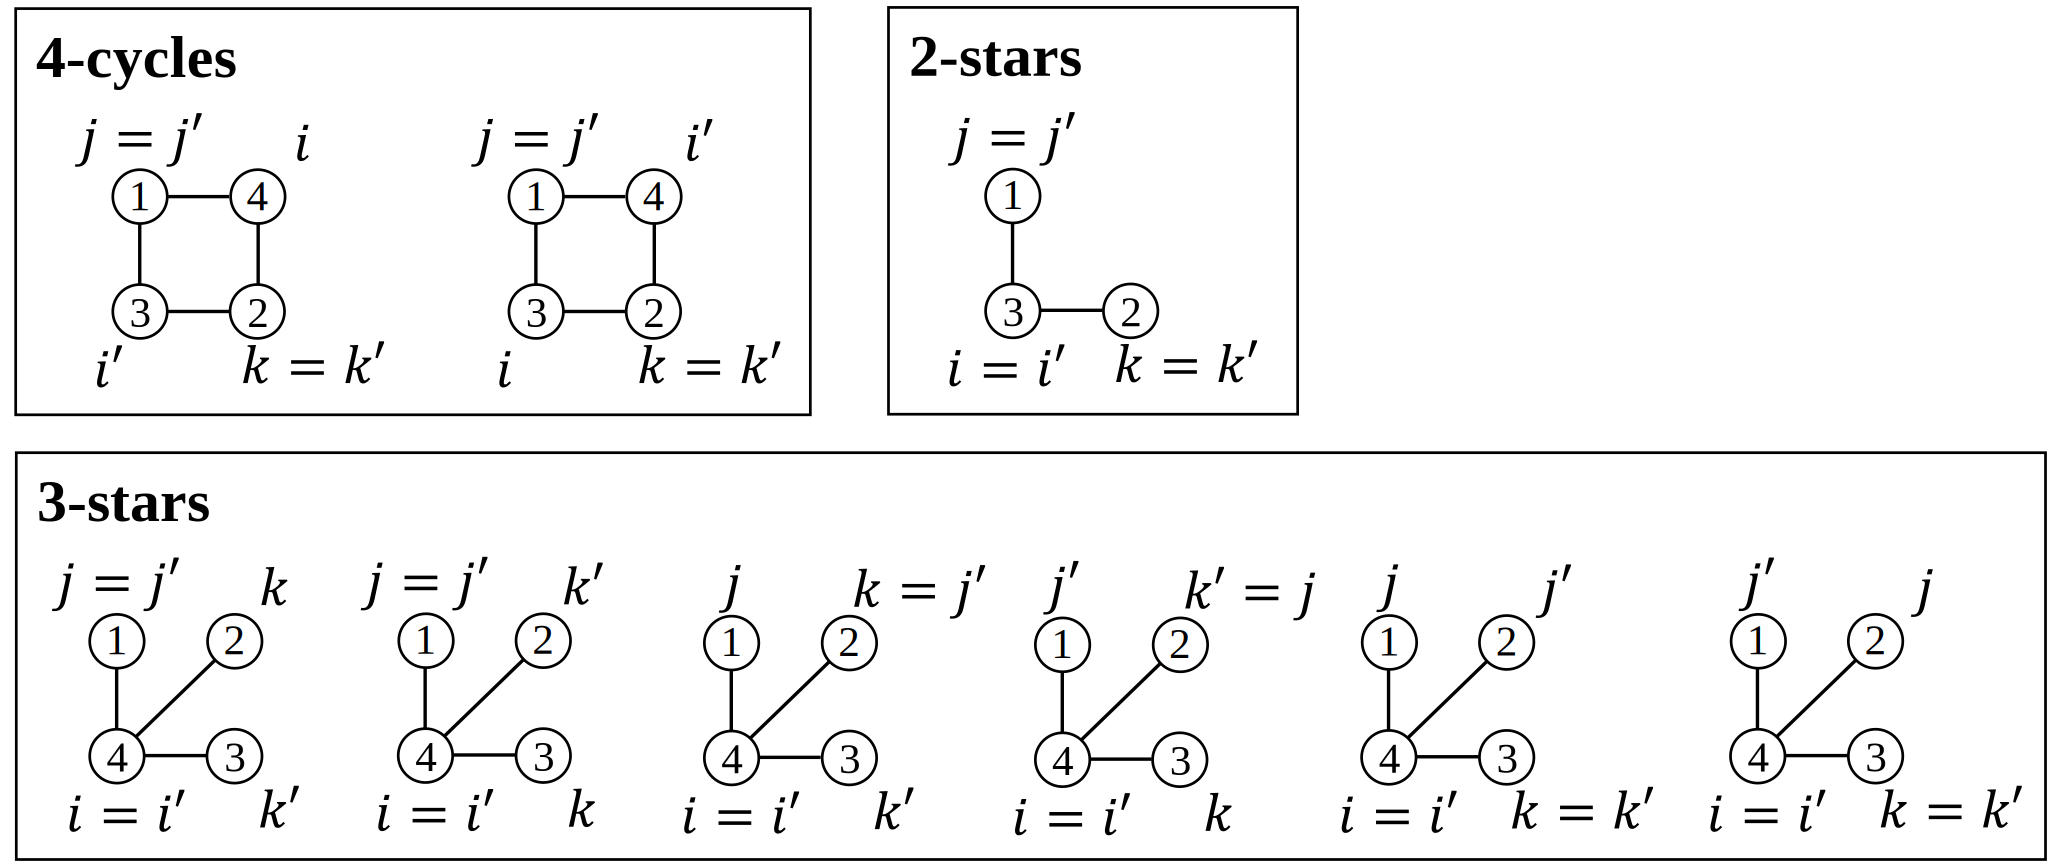
\includegraphics[width=0.99\linewidth]{fig/associated_subgraphs.pdf}
  
  \caption{Examples of two 4-cycles, six 3-stars, and one 2-stars.}
  \label{chap2-fig:associated_subgraphs}
\end{figure}

In the following, let $P(i,j,k)$ be the event that $F_{ijk} = F_{i'j'k'} = 1$.
Observing Figure~\ref{chap2-fig:four-cycle}, we can see that in both possible ways in
which a valid choice maps to a $4$-cycle, then $P(i,j,k)$ holds when at least $3$
edges in $E'$ are present. Each edge in $E'$ is independent,
and is present with probability at most $\mu$. Thus, $\Pr[P(i,j,k)] \leq \mu^3$.
Next, if a valid choice maps to a $3$-star, then $P(i,j,k)$ implies at least $3$
edges in $E'$ are present. Thus, $\Pr[P(i,j,k) = 1] \leq \mu^3$.
Finally, if a valid choice maps to a $2$-star, then $P(i,j,k) = 1$
if and only if $2$ edges in $E'$ are present. Thus, $\Pr[P(i,j,k) = 1] \leq \mu^2$.

Putting this together,
\[
  \V\left[\sum_{i=1}^n w_i\right] \leq 2 C_4(G) \mu^3 + 6 S_3(G) \mu^3 + S_2(G) \mu^2.
\]
Plugging into~\eqref{chap2-eq:inter_var}, we get
% \[
\begin{align*}
  &\;\V[\hf_\triangle(G)] \\
  &\leq \frac{1}{(1-\rho)^2} \left(\frac{1}{\mu}(2C_4(G) + 6S_3(G)) + \frac{1}{\mu^2} S_2(G) + 2n\frac{d_{max}^2}{\mu^4\epsilon_2^2}\right).
% \]
\end{align*}
This establishes the result. \qed

\smallskip
\noindent{\textbf{Bounding the Variance in \AlgThree{}.}}~~In \AlgThree{}, for a fixed
$v_i \in V$, we have $(v_j, v_k) \in M_i$ if and only if
$j < k < i$, $(v_j, v_k) \in E'$, $(v_i, v_k) \in E'$, and $(v_i, v_k) \in E'$
from~\eqref{chap2-eq:M_i_III}. Thus,
\begin{align*}
\sum_{i=1}^n w_i &= \sum_{i=1}^n~\sum_{\substack{1 \leq j < k < i \leq n \\
a_{i,j} = 1, a_{i,k} = 1}} \textbf{1}_{(v_j, v_k) \in M_i} \\
&= \sum_{1 \leq j < k < i \leq n}
a_{i,j}a_{i,k}\textbf{1}_{(v_j, v_k) \in E'} \textbf{1}_{(v_i, v_k) \in E'}\textbf{1}_{(v_j, v_k) \in E'}.
\end{align*}

Define the random variable $F_{ijk} = \textbf{1}_{(v_j v_k) \in E'}
\textbf{1}_{(v_i, v_k) \in E'} \allowbreak \textbf{1}_{(v_j, v_k) \in E'}$. Following the same
steps as those in the proof of \AlgTwo{}, we have
\begin{align*}
  \V\left[\sum_{i=1}^n w_i\right]
  &= \sum_{\substack{1 \leq j < k < i \leq n \\ 1 \leq j' < k' <
  i' \leq n}} a_{i,j} a_{i,k} a_{i',j'} a_{i',k'} \cov(F_{ijk}, F_{i'j'k'}) \\
  &\leq
  \sum_{i,i',j,j',k,k'\text{ valid}} \Pr[F_{ijk} = F_{i'j'k'} = 1].
\end{align*}

As we showed in the proof for \AlgTwo{}, each $4$-cycle of $G$ has at most
2 valid choices mapped to it, each $3$-star of $G$ has at most 6 valid
choices mapped to it, and each $2$-star of $G$ has at most one valid choice
mapped to it.

In the following, let $P(i,j,k)$ be the event that $F_{ijk} = F_{i'j'k'} = 1$.
Observing Figure~\ref{chap2-fig:four-cycle}, we can see that for each possible
mapping of a valid choice to a $4$-cycle, five edges must be present in $G'$ in
order for $P(i,j,k) = 1$. Thus, $\Pr[P(i,j,k) = 1] \leq \mu^5$. For each possible
mapping of a valid choice to a $3$-star, five edges must be present in $G'$ in
order for $P(i,j,k) = 1$. Thus, $\Pr[P(i,j,k) = 1] \leq \mu^5$. For each possible
mapping of a valid choice to a $2$-star, three edges must be present in $G'$ in
order for $P(i,j,k) = 1$. Thus, $\Pr[P(i,j,k) = 1] \leq \mu^3$.

Plugging into~\eqref{chap2-eq:inter_var}, we get
% \[
\begin{align*}
  &\;\V[\hf_\triangle(G)] \\
  &\leq \frac{1}{(1-\rho)^2} \left(\frac{1}{\mu}(2C_4(G) + 6S_3(G)) + \frac{1}{\mu^3} S_2(G) + 2n\frac{d_{max}^2}{\mu^6\epsilon_2^2}\right).
% \]
\end{align*}
This establishes the result.
\qed

\begin{lemma}
  \label{chap2-lem:c_ij_4cycle_2star}
  Let $c_{ij} = \sum_{l < i \leq n} a_{l,i} a_{l,j}$. Then,
\[
    \sum_{i,j=1, i<j}^n c_{ij}^2 \leq 2 C_4(G) + S_2(G).
\]
\end{lemma}
\begin{proof}
  \begin{align*}
      \sum_{i,j=1, i<j}^n c_{ij}^2
      &= \sum_{i,j=1, i<j}^n c_{ij} + \sum_{i,j=1, i<j}^n c_{ij}(c_{ij}-1) \\
      &= S_2(G) + \sum_{i,j=1, i<j}^n c_{ij}(c_{ij}-1).
  \end{align*}
  Let $C_{i-*-j-*-i}(G)$ be the number of 4-cycles in $G$
  %that starts with $i$ and reaches $j$ after two hops.
  such that the first and third nodes are $v_i$ and $v_j$, respectively $(i<j)$, and the remaining two nodes have smaller indices than $i$.
  From middle nodes in 2-paths starting at $v_i$ and ending at $v_j$, we can choose two nodes as the second and fourth nodes in the 4-cycles.
  $c_{ij}$ is the number of nodes that have smaller IDs than $v_i$ and are connected to $v_i$ and $v_j$.
  Thus,
  $C_{i-*-j-*-i}(G) = \binom{c_{ij}}{2}$.
  Therefore, we have
  \begin{align*}
      \sum_{i,j=1, i<j}^n c_{ij}^2
       &= S_2(G) + \sum_{i,j=1, i<j}^n 2C_{i-*-j-*-i}(G) \\
      &\leq S_2(G) + 2 C_4(G).
  \end{align*}
The last inequality comes from the fact that
two nodes with the largest indices may not be opposite to each other in some 4-cycles in $G$.
\end{proof}

\section{Proof of Statements in Section~\ref{chap2-sec:double_clip}}
\label{chap2-sec:proof_double_clip}
\subsection{Proof of Theorem~\ref{chap2-thm:privacy_DC}}

Let $\bma_i, \bma'_i \in \{0,1\}^n$ be two neighbor lists that differ in one bit.
Let ${t_i}'$, $s'_i$, and ${w_i}'$ be respectively the values of $t_i$ (in line 8 of Algorithm~\ref{chap2-alg:clip}), $s_i$ (in line 9), and $w_i$ (in line 10) when the neighbor list of user $v_i$ is $\bma'_i$.
Let $\Delta w_i = |{w_i}' - w_i|$.

We assume that $|\bma'_i| = |\bma_i| + 1$ without loss of generality.
Let $\bar{\bma}_i, \bar{\bma}'_i \in \{0,1\}^n$ be neighbor lists corresponding to $\bma_i$ and $\bma'_i$, respectively, after edge clipping.
Note that $|\bar{\bma}_i| = |\bar{\bma}'_i| \leq \td_i$.
There are three cases for $\bar{\bma}_i$ and $\bar{\bma}'_i$:
\begin{enumerate}
    \item $\bar{\bma}_i$ is identical to $\bar{\bma}'_i$ and $|\bar{\bma}_i| = |\bar{\bma}'_i| = \td_i$.
    \item $\bar{\bma}_i$ and $\bar{\bma}'_i$ differ in one bit and $|\bar{\bma}'_i| = |\bar{\bma}_i| + 1$.
    \item $\bar{\bma}_i$ and $\bar{\bma}'_i$ differ in two bits and $|\bar{\bma}_i| = |\bar{\bma}'_i| = \td_i$.
\end{enumerate}
Note that the third case can happen when $|\bma'_i| \geq \td_i$.
For example, assume that $n=8$, $\td_i=4$, $\bma_i=(1,1,0,1,0,1,1,1)$ and $\bma'_i=(1,1,1,1,0,1,1,1)$.
If we select four ``1''s in the order of 3, 1, 4, 6, 8, 2, 7, and 5-th bit in the neighbor list,
$\bar{\bma}_i$ and $\bar{\bma}'_i$ will be:
$\bar{\bma}_i=(1,0,0,1,0,1,0,1)$ and $\bar{\bma}'_i=(1,0,1,1,0,1,0,0)$,
which differ in two bits.

If $\bar{\bma}_i$ and $\bar{\bma}'_i$ differ in one bit ($|\bar{\bma}'_i| = |\bar{\bma}_i| + 1$), then ${t_i}' - t_i \in [0,\kappa_i]$ and $s'_i - s_i \in [0,\td_i]$, hence $\Delta w_i = |({t_i}' - t_i) - \mu^*\rho(s'_i - s_i)| \leq \kappa_i$.
If $\bar{\bma}_i$ and $\bar{\bma}'_i$ differ in two bits ($|\bar{\bma}_i| = |\bar{\bma}'_i| = d_{max}$), then ${t_i}' - t_i \in [-\kappa_i,\kappa_i]$ and $s_i = s'_i = \binom{\td_i}{2}$, hence $\Delta w_i \leq \kappa_i$.

Therefore, we always have $\Delta w_i \leq \kappa_i$
(if $\bar{\bma}_i$ is identical to $\bar{\bma}'_i$, $\Delta w_i =0$).
Since we add $\Lap(\frac{1}{\epsilon_0})$
to $d_i$ and
$\Lap(\frac{\kappa_i}{\epsilon_2})$
to $w_i^*$, the second round provides ($\epsilon_0+\epsilon_2$)-edge LDP.
The first round provides $\epsilon_1$-edge LDP and we use only the lower-triangular part of $\bmA$.
Thus, by sequential composition (Proposition~\ref{chap2-prop:seq_comp_edge_LDP}) 
and Proposition~\ref{chap2-prop:edge_LDP_entire_edge_LDP},
$\calR_i$ satisfies $(\epsilon_0 + \epsilon_1 + \epsilon_2)$-edge LDP, and $(\calR_1, \ldots, \calR_n)$ satisfies $(\epsilon_0 + \epsilon_1 + \epsilon_2)$-relationship DP.
\qed

\subsection{Proof of Theorem~\ref{chap2-thm:triangle_excess}}

Recall that
$t_{i,j} = |\{(v_i,v_j,v_k) : a_{i,k} = 1, (v_j,v_k) \in M_i, j<k<i \}|$.
Let
$t'_{i,j} = |\{(v_i,v_j,v_k) : a_{i,k} = 1, (v_j,v_k) \in M_i \}|$.
Then $t_{i,j} \leq t'_{i,j}$.
Thus we have
\begin{align*}
    \Pr(t_{i,j} > \kappa_i) \leq \Pr(t_{i,j} \geq \kappa_i) \leq \Pr(t'_{i,j} \geq \kappa_i).
\end{align*}

Below we first prove (\ref{chap2-eq:AlgI_clip_bound}) and (\ref{chap2-eq:AlgII_clip_bound}). Then we prove (\ref{chap2-eq:AlgIII_clip_bound}).

\smallskip
\noindent{\textbf{Proof of (\ref{chap2-eq:AlgI_clip_bound}) and (\ref{chap2-eq:AlgII_clip_bound}).}}~~For each edge $(v_i,v_j)$, we have $\sum_{k \ne i,j} \textbf{1}_{(v_i,v_k) \in E} \leq \td_i$.
% In addition, each edge $(v_j,v_k)$ is included in $E'$ with probability at most $\mu^*$, and all the events are independent in \AlgOne{} and \AlgTwo{}.
In \AlgOne{}, each edge $(v_j,v_k)$ is included in $E'$ with probability at most $\mu$, and all the events are independent.
In \AlgTwo{}, each of the edges $(v_i,v_k)$ and $(v_j,v_k)$ is included in $E'$ with probability at most $\mu$, and all the events are independent.
Thus, $\Pr(t'_{i,j} \geq \kappa_i)$ is less than or equal to the probability that the number of successes in the binomial distribution $B(\td_i, \mu^*)$ ($\mu^* = \mu$ in \AlgOne{} and $\mu^2$ in \AlgTwo{}) is larger than or equal to $\kappa_i$.

Let $X_{n,p}$ be a random variable representing the number of successes in the binomial distribution $B(n,p)$, and $F(\kappa_i;n,p) = \Pr(X_{n,p} \leq \kappa_i)$; i.e., $F$ is a cumulative distribution function of $B(n,p)$.
Since $\kappa_i \geq \mu^* \td_i$, we have
\begin{align*}
    &\Pr(t'_{i,j} \geq \kappa_i) \\
    &\leq \Pr(X_{\td_i, \mu^*} \geq \kappa_i) \\
    &= F(\td_i - \kappa_i; \td_i, 1-\mu^*) \\
    &\leq \exp \left[-\td_i D \left(\frac{\td_i - \kappa_i}{\td_i} \parallel 1-\mu^* \right) \right]  \text{(by Chernoff bound)}\\
    &= \exp \left[-\td_i D \left(\frac{\kappa_i}{\td_i} \parallel \mu^* \right) \right],
\end{align*}
which proves (\ref{chap2-eq:AlgI_clip_bound}) and (\ref{chap2-eq:AlgII_clip_bound}) (as $\Pr(t_{i,j} > \kappa_i) \leq \Pr(t'_{i,j} \geq \kappa_i)$).

\smallskip
\noindent{\textbf{Proof of (\ref{chap2-eq:AlgIII_clip_bound}).}}~~Assume that $\kappa_i \geq \mu^2 \td_i$ in \AlgThree{}.
For each edge $(v_i,v_j)$, we have $\sum_{k \ne i,j} \textbf{1}_{(i,k) \in E} \leq \td_i$.
In addition, each of the edges $(v_i,v_k)$ and
$(v_j,v_k)$ are included in $E'$ with probability at most $\mu$, and all the events are independent.

If $(v_i,v_j)$ is included in $E'$ (which happens with probability at most $\mu$), $\Pr(t'_{i,j} \geq \kappa_i)$ is less than or equal to the probability that the number of successes in the binomial distribution $B(\td_i, \mu^2)$ is larger than or equal to $\kappa_i$.
Otherwise (i.e., if $(v_i,v_j)$ is not included in $E'$), then $t'_{i,j} = 0$.

Thus, if $\kappa_i \geq \mu^2 \td_i$, we have
\begin{align*}
    &\Pr(t'_{i,j} \geq \kappa_i) \\
    &\leq \mu \Pr(X_{\td_i, \mu^2} \geq \kappa_i) \\
    &= \mu F(\td_i - \kappa_i; \td_i, 1-\mu^2) \\
    &\leq \mu \exp \left[-\td_i D \left(\frac{\td_i - \kappa_i}{\td_i} \parallel 1-\mu^2 \right) \right]  ~ \text{(by Chernoff bound)}\\
    &= \mu \exp \left[-\td_i D \left(\frac{\kappa_i}{\td_i} \parallel \mu^2 \right) \right],
\end{align*}
and therefore (\ref{chap2-eq:AlgIII_clip_bound}) holds (as $\Pr(t_{i,j} > \kappa_i) \leq \Pr(t'_{i,j} \geq \kappa_i)$).


If $\mu^3 \td_i \leq \kappa_i < \mu^2 \td_i$, (\ref{chap2-eq:AlgIII_clip_bound}) can be written as: $\Pr(t_{i,j} > \kappa_i) \leq \mu \exp \left[-\td_i D \left(\mu^2 \parallel \mu^2 \right) \right] = \mu$.
This clearly holds because each edge $(v_i,v_j)$ is included in $E'$ with probability at most $\mu$.
\qed
}
